% appendix.tex
\chapter{Appendix}

\section{Database SQL Tests}

\begin{figure}[H]
    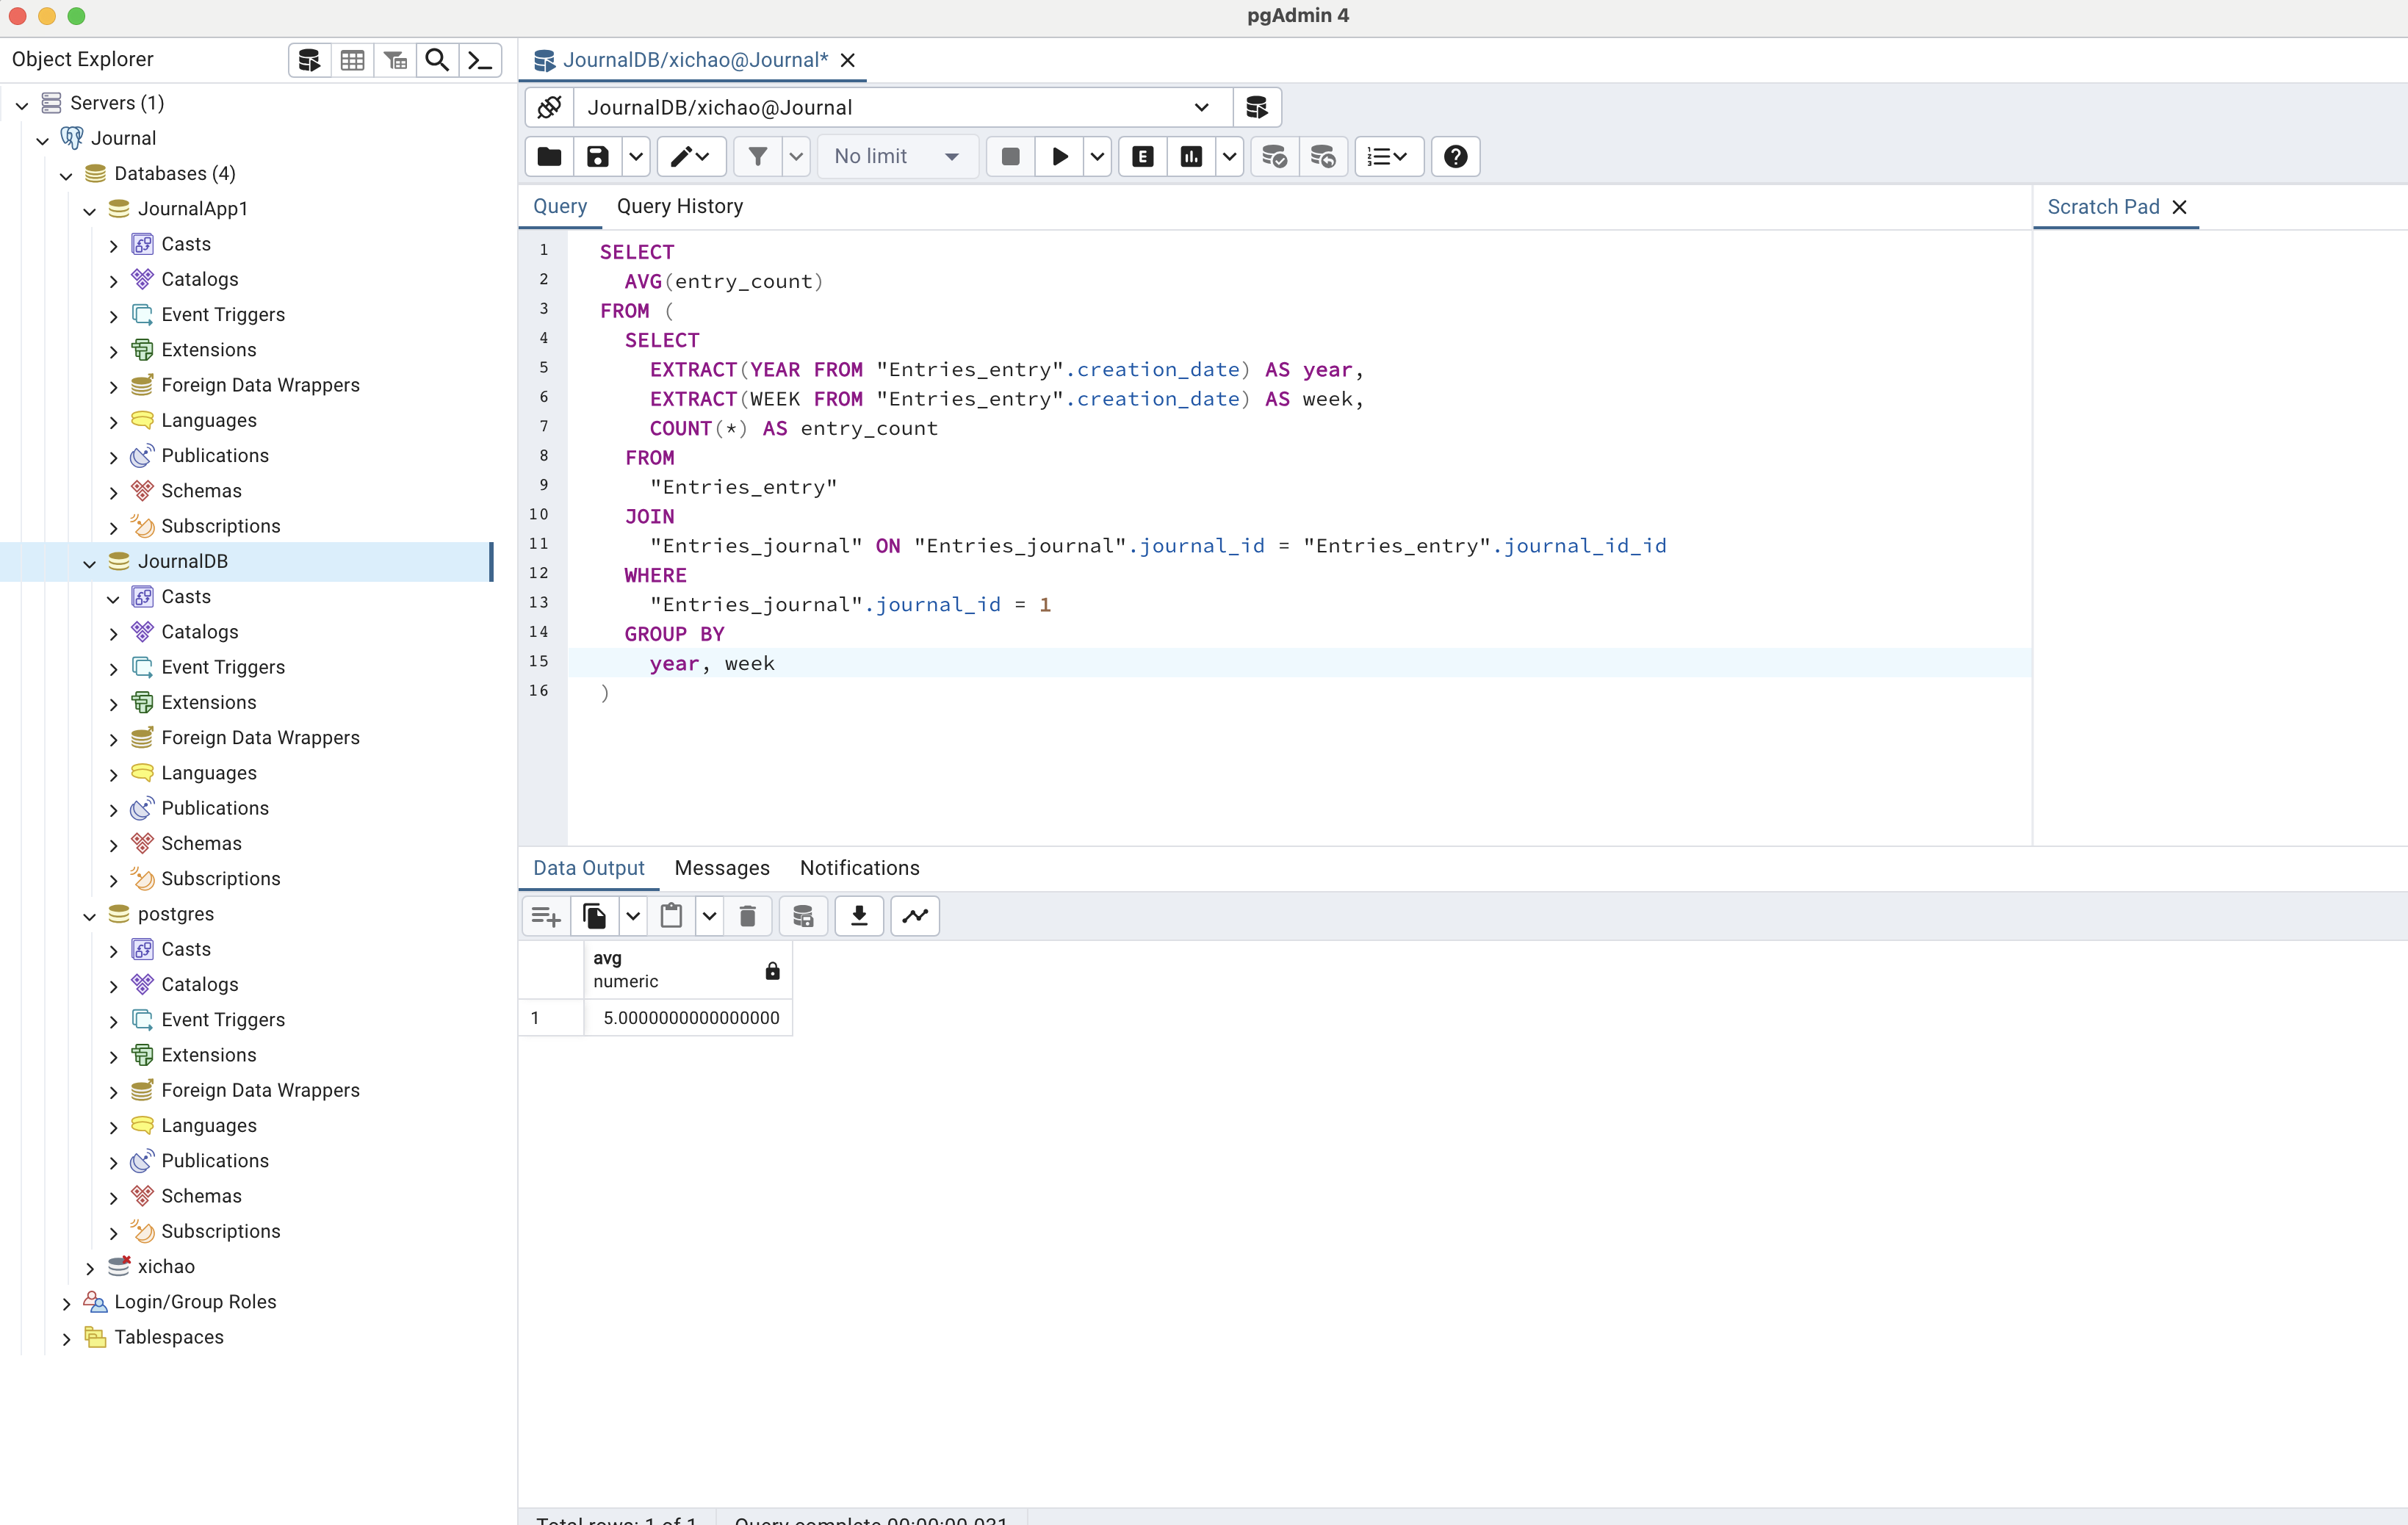
\includegraphics[width=\textwidth]{Assets/test_average_entry_per_week.png}
    \caption{Query result for average entry per week.}
    \label{fig:average_entry_per_week}
\end{figure}

\begin{figure}[H]
    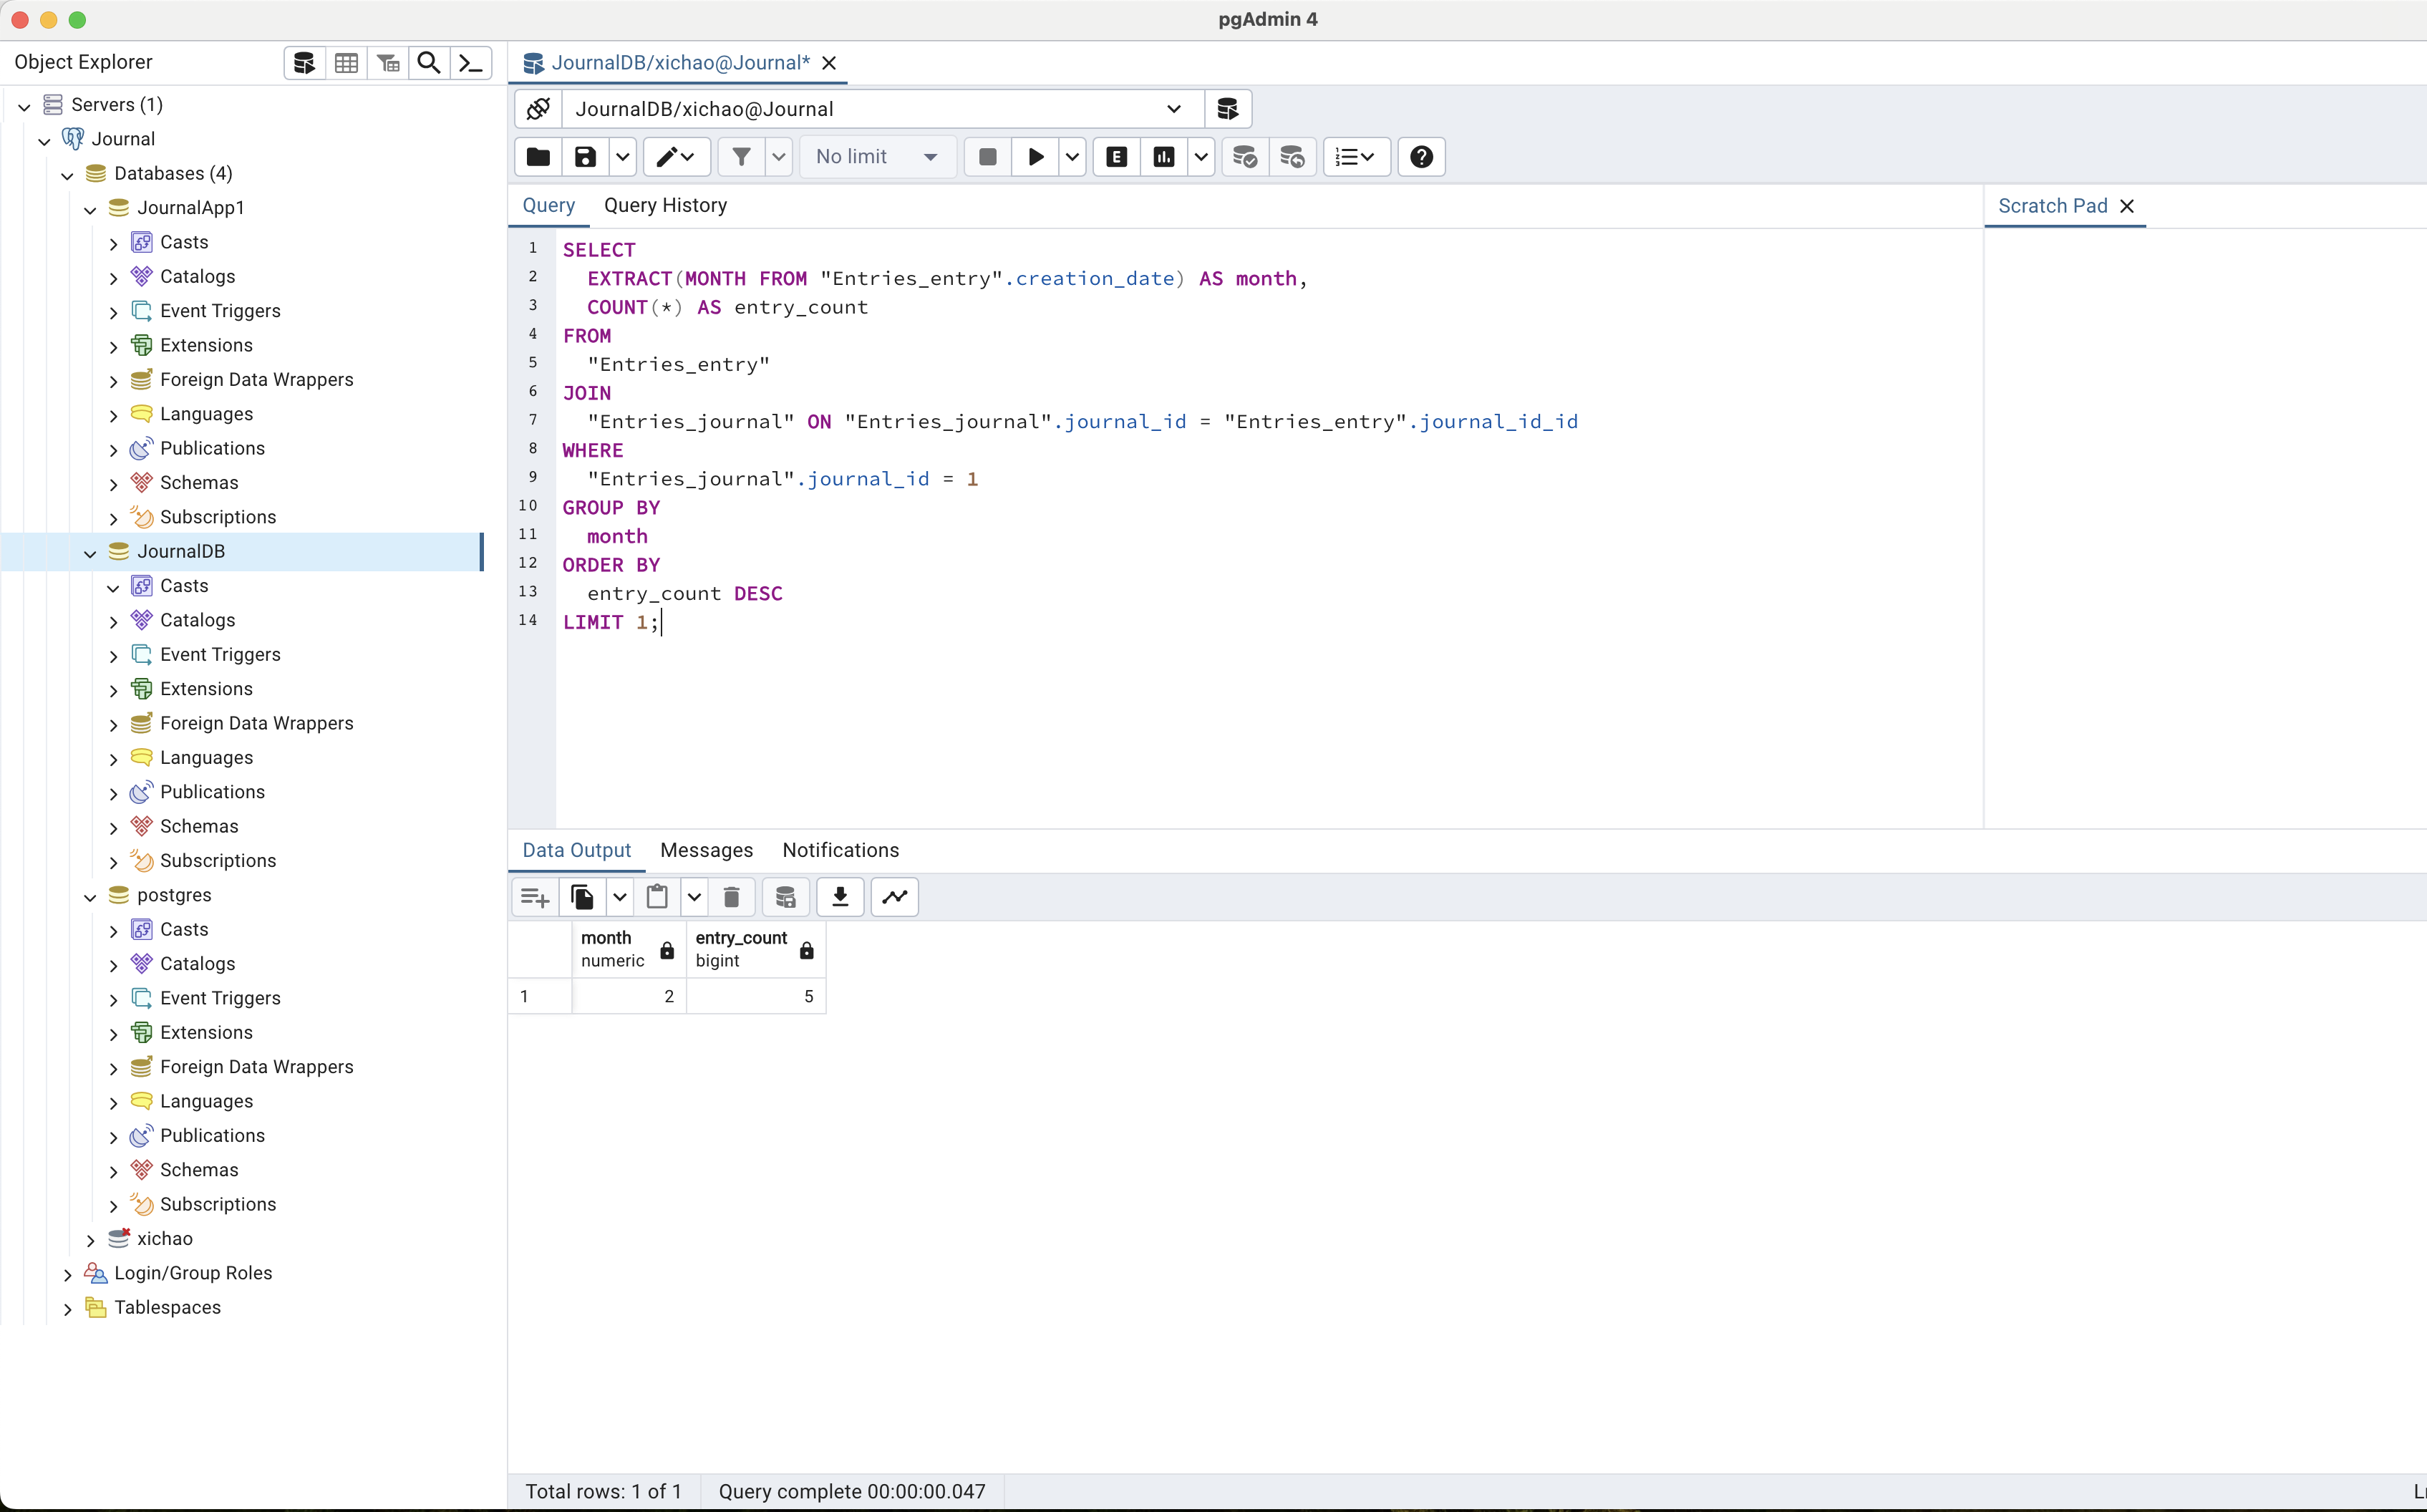
\includegraphics[width=\textwidth]{Assets/test_most_active_month.png}
    \caption{Query result for most active month.}
    \label{fig:most_active_month}
\end{figure}

\begin{figure}[H]
    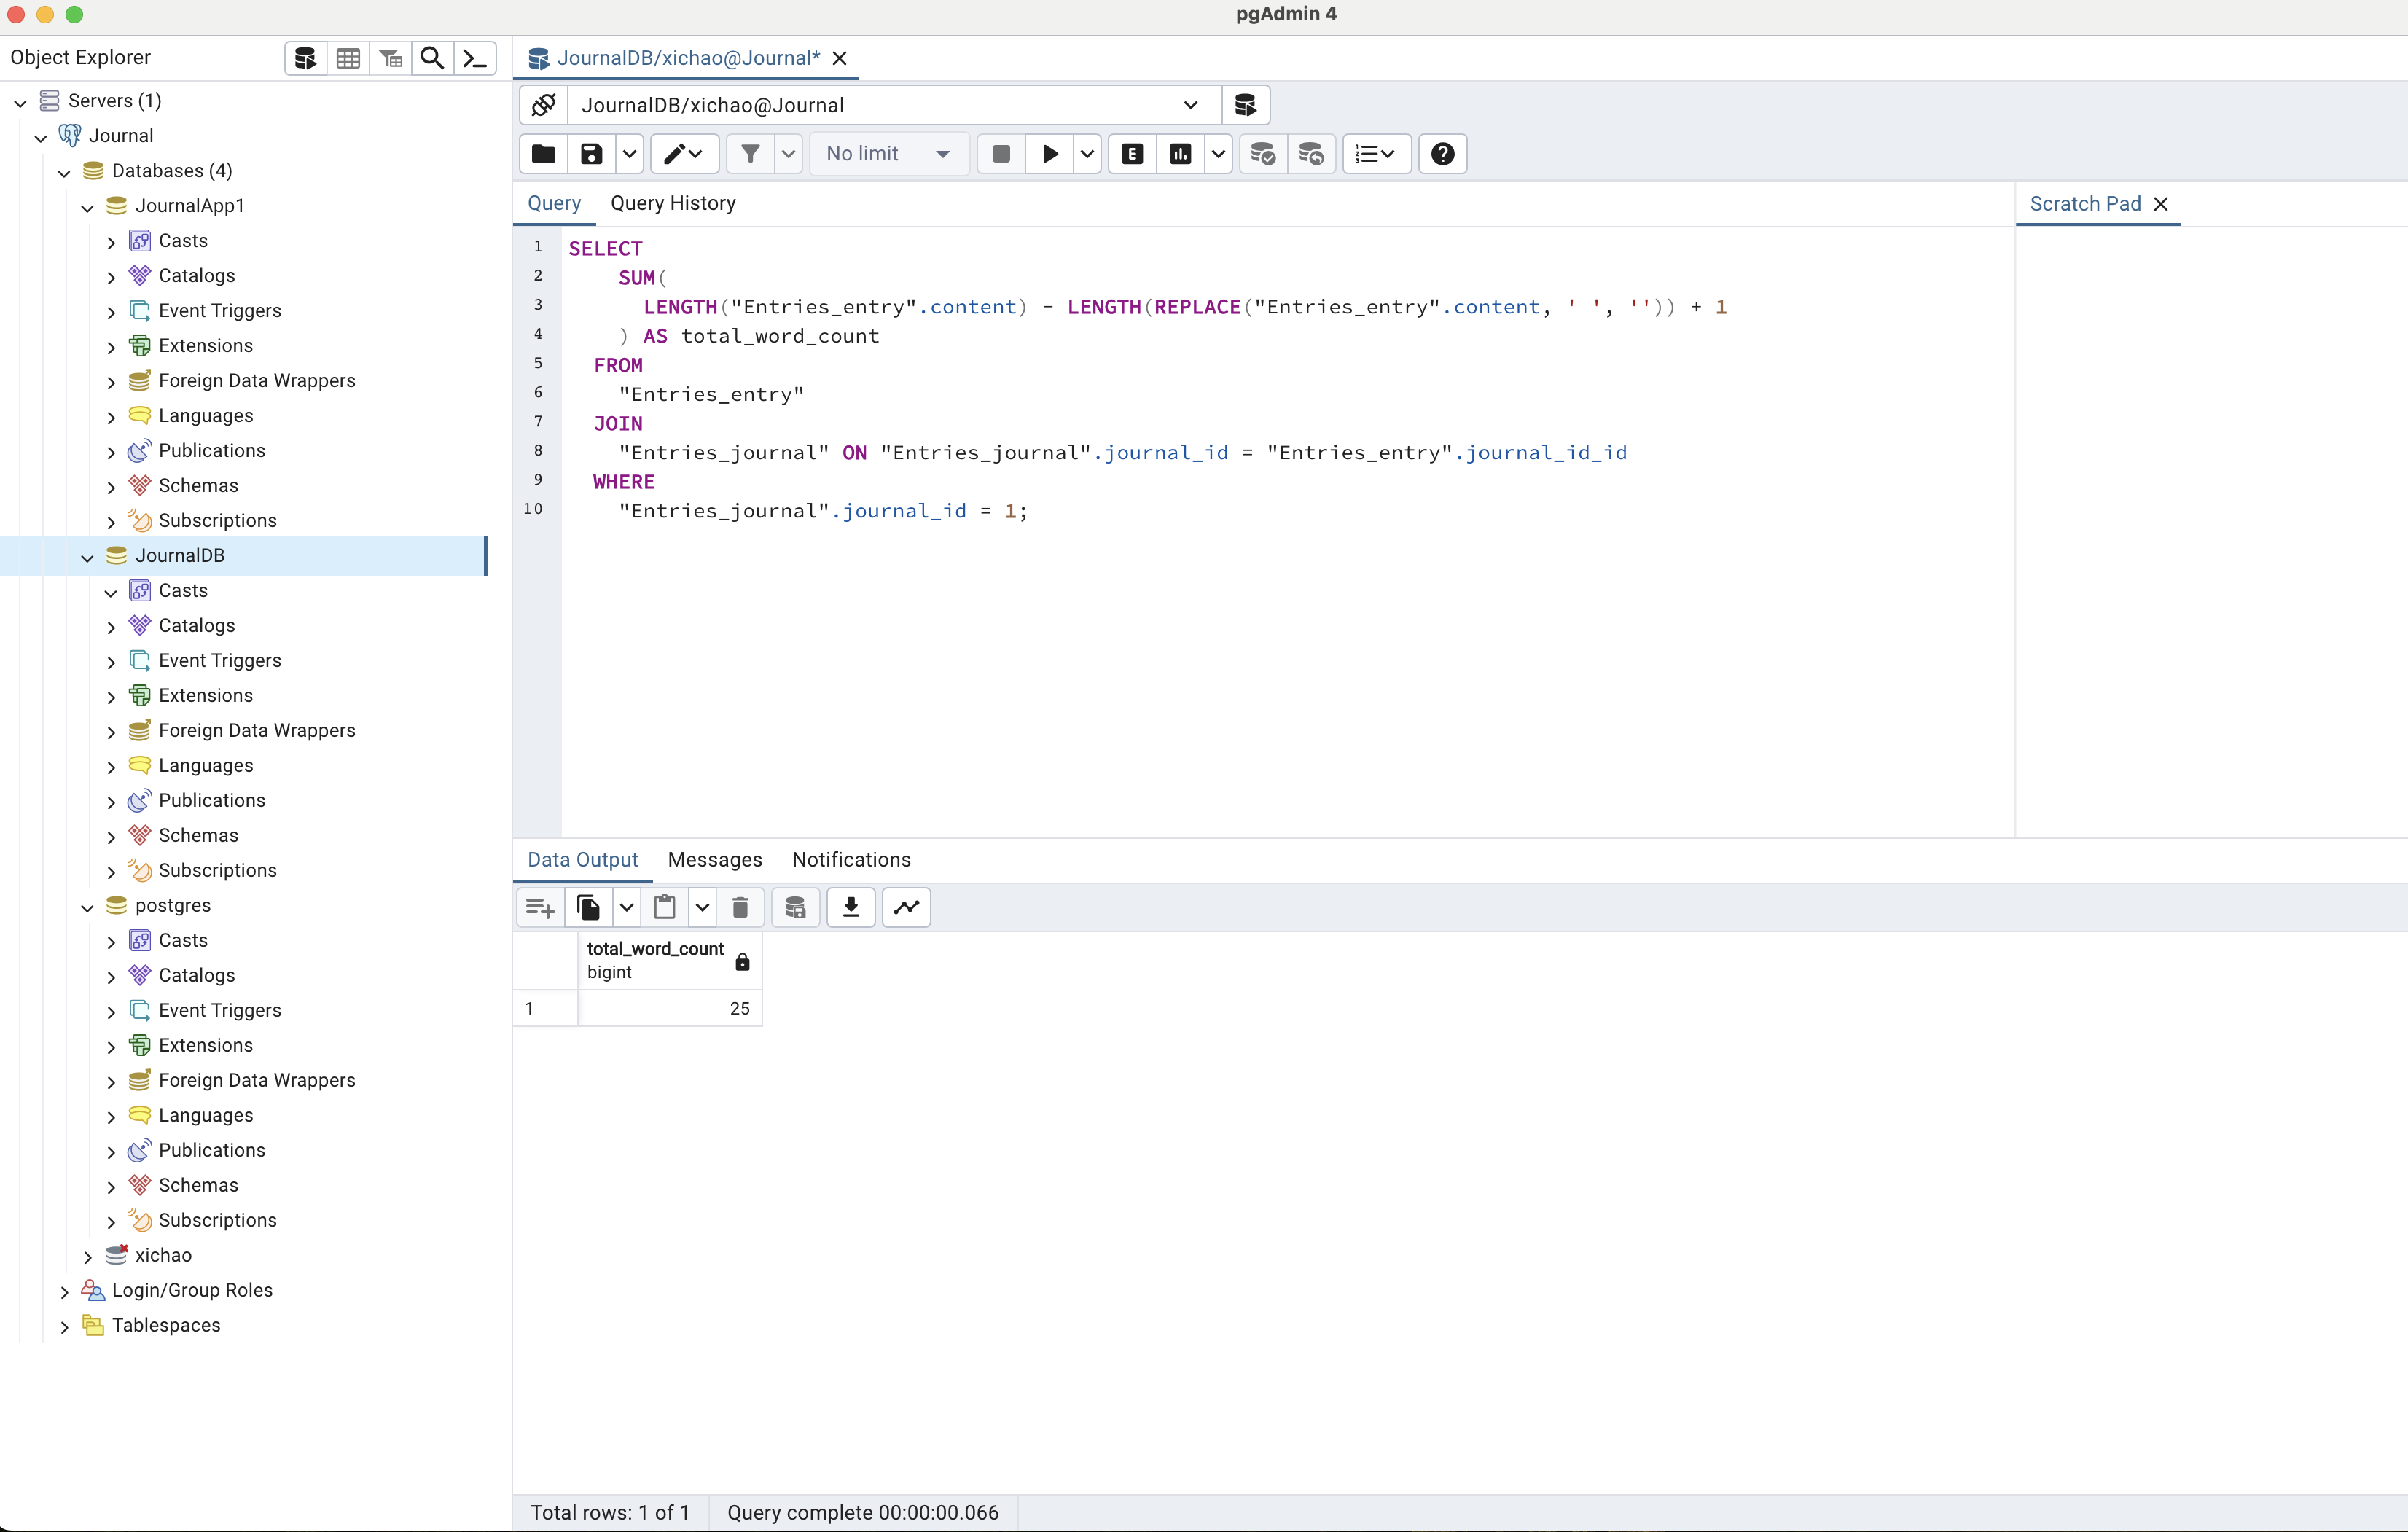
\includegraphics[width=\textwidth]{Assets/test_total_word_count.png}
    \caption{Query result for total word count.}
    \label{fig:total_word_count}
\end{figure}


\section{API Test Details}

\subsection{User App}
\subsection{register/}
\begin{figure}[H]
    \caption{Request to register a new user that already exists}
    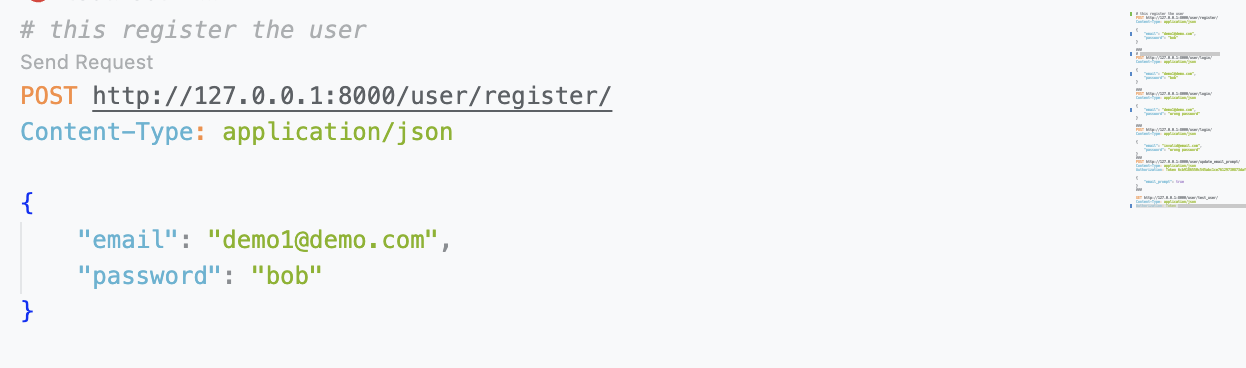
\includegraphics[width=\textwidth]{Assets/api_test/request_register_already_exist.png}
    \label{fig:request_register_already_exist}
\end{figure}

\begin{figure}{H}
    \caption{Response to register a new user that already exists}
    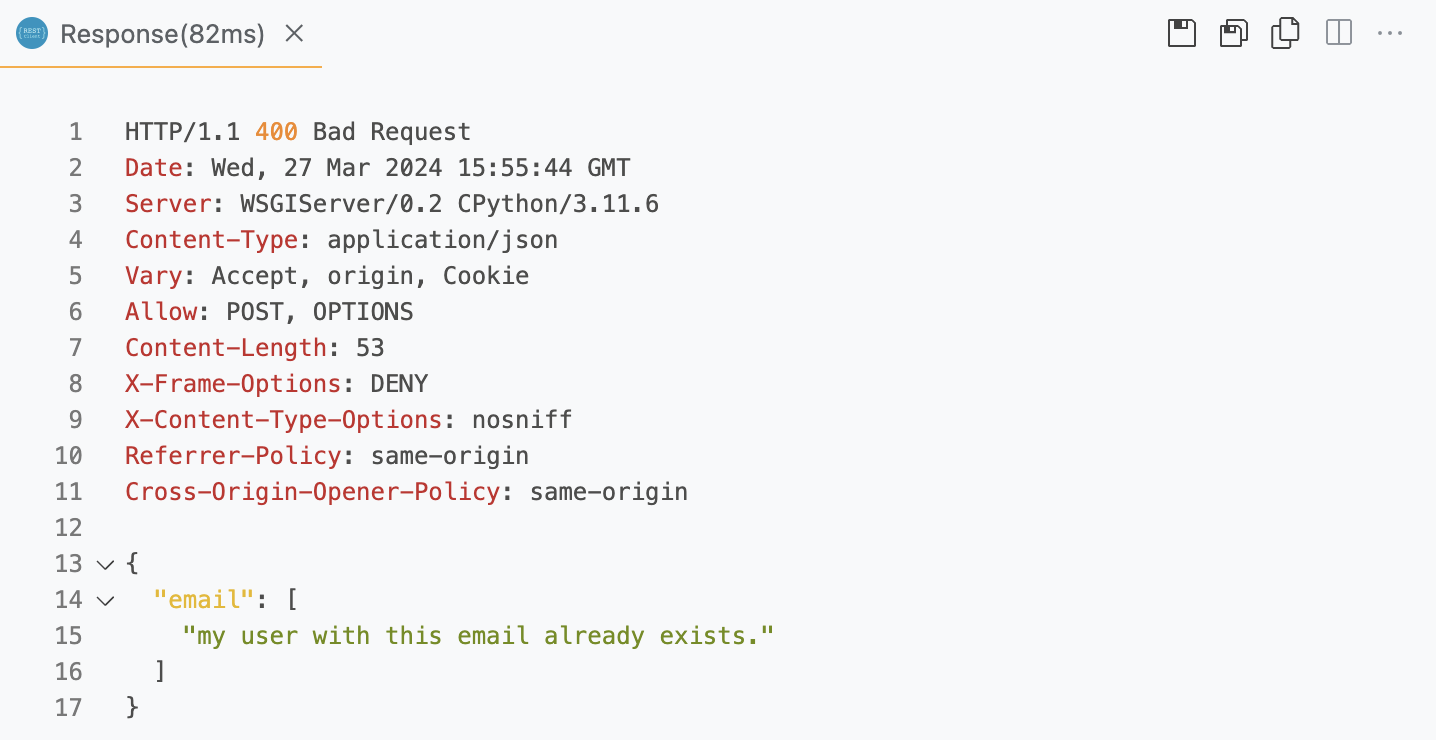
\includegraphics[width=\textwidth]{Assets/api_test/response_register_already_exist.png}
    \label{fig:response_register_already_exist}
\end{figure}

\begin{figure}[H]
    \caption{Request to register a new user that does not exist}
    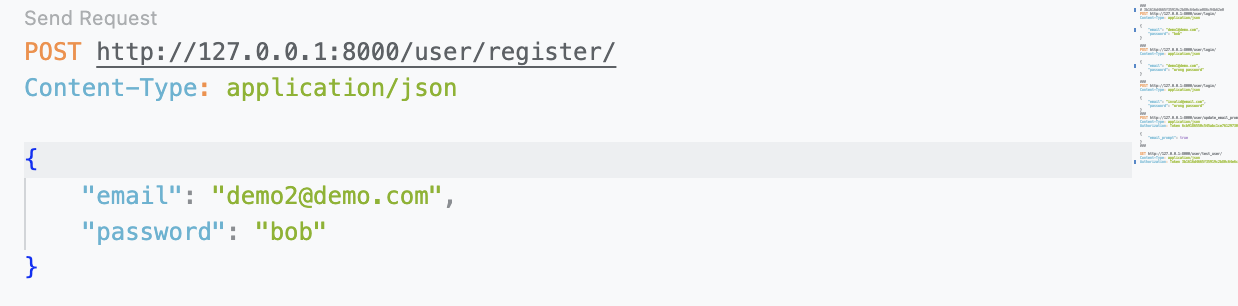
\includegraphics[width=\textwidth]{Assets/api_test/request_register_sucess.png}
    \label{fig:request_register_new_user}
\end{figure}

\begin{figure}[H]
    \caption{Response to register a new user that does not exist}
    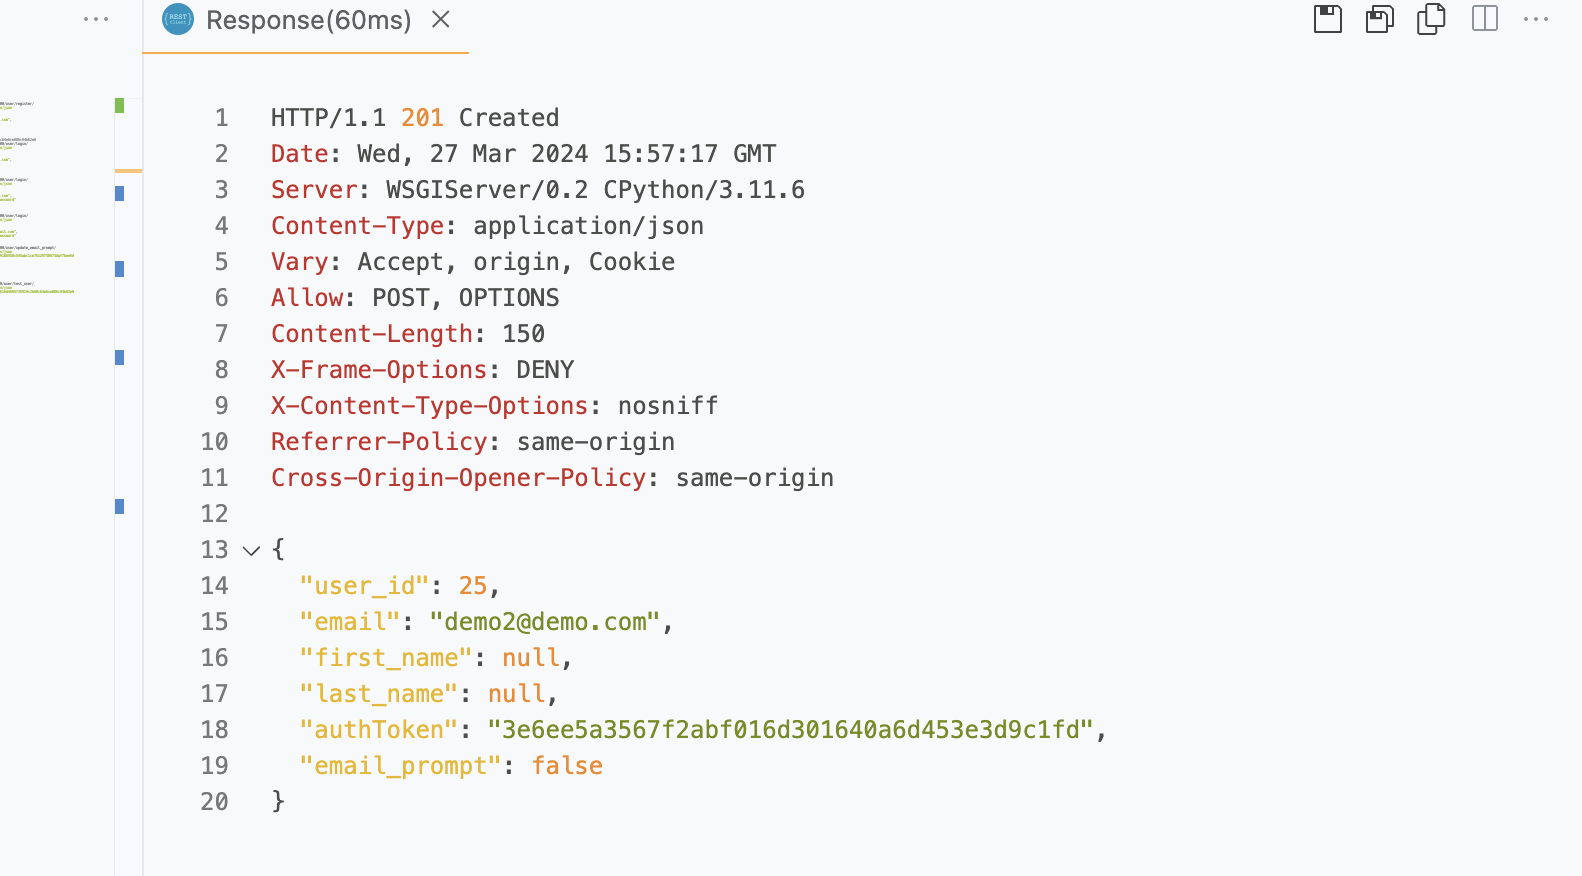
\includegraphics[width=\textwidth]{Assets/api_test/response_register_sucess.png}
    \label{fig:response_register_new_user}
\end{figure}

\begin{figure}[H]
    \caption{Request to register a new user with an invalid email}
    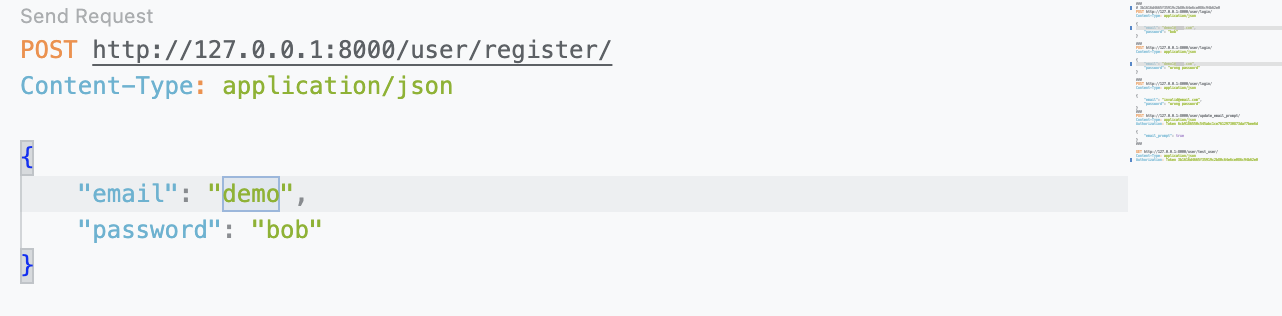
\includegraphics[width=\textwidth]{Assets/api_test/request_register_invalid_email.png}
    \label{fig:request_register_invalid_email}
\end{figure}

\begin{figure}[H]
    \caption{Response to register a new user with an invalid email}
    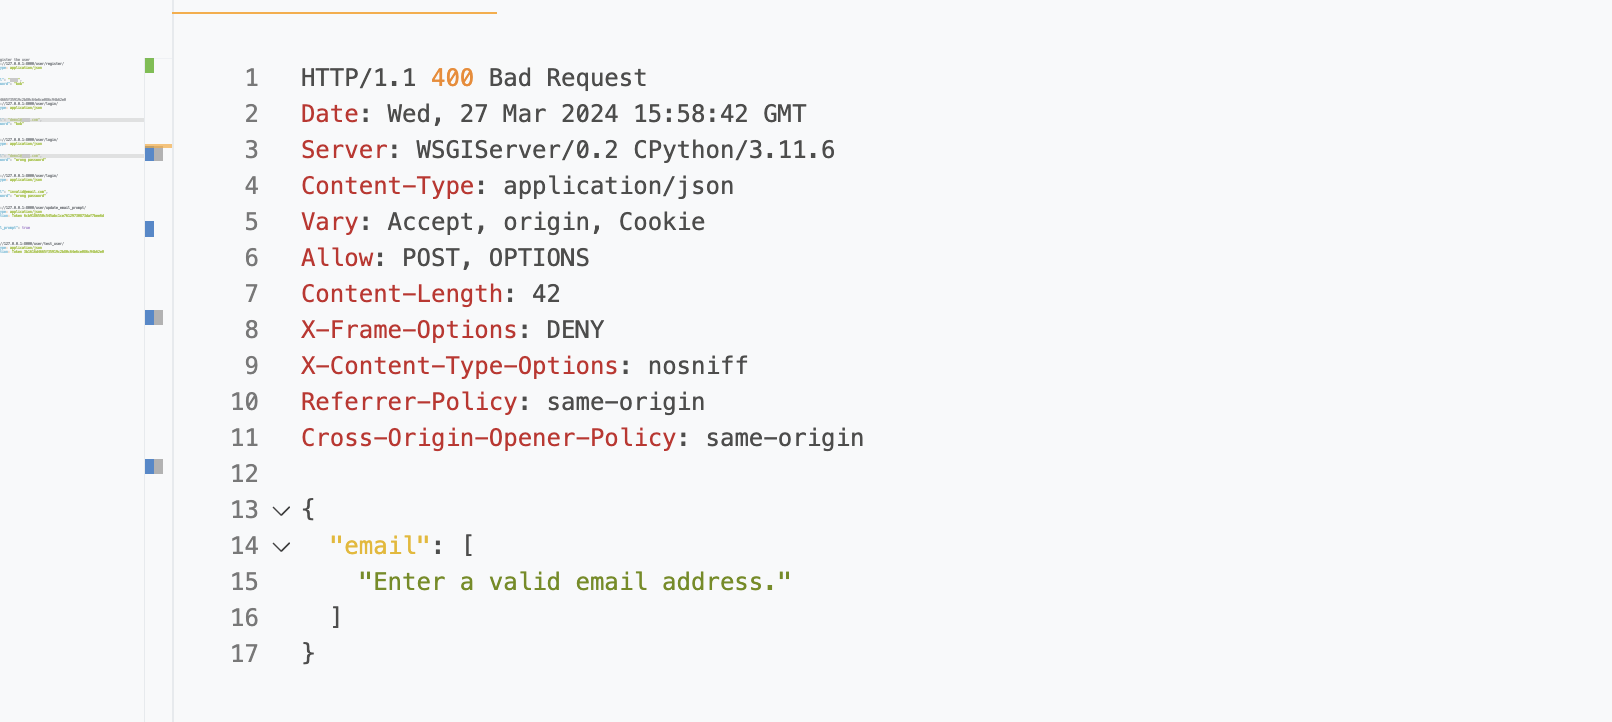
\includegraphics[width=\textwidth]{Assets/api_test/response_register_invalid_email.png}
    \label{fig:response_register_invalid_email}
\end{figure}

\subsection{login/}
\begin{figure}[H]
    \caption{Request to login with a valid user}
    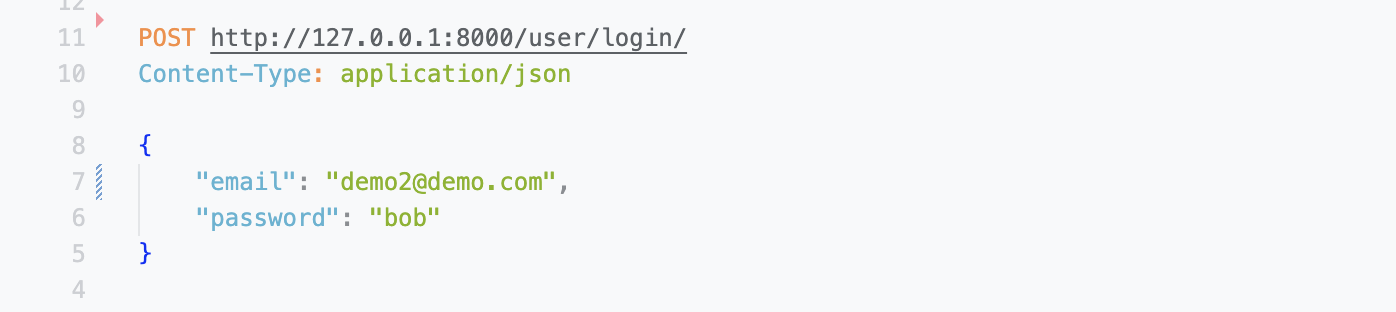
\includegraphics[width=\textwidth]{Assets/api_test/request_login_sucessful.png}
    \label{fig:request_login_sucessful}
\end{figure}

\begin{figure}[H]
    \caption{Response to valid login}
    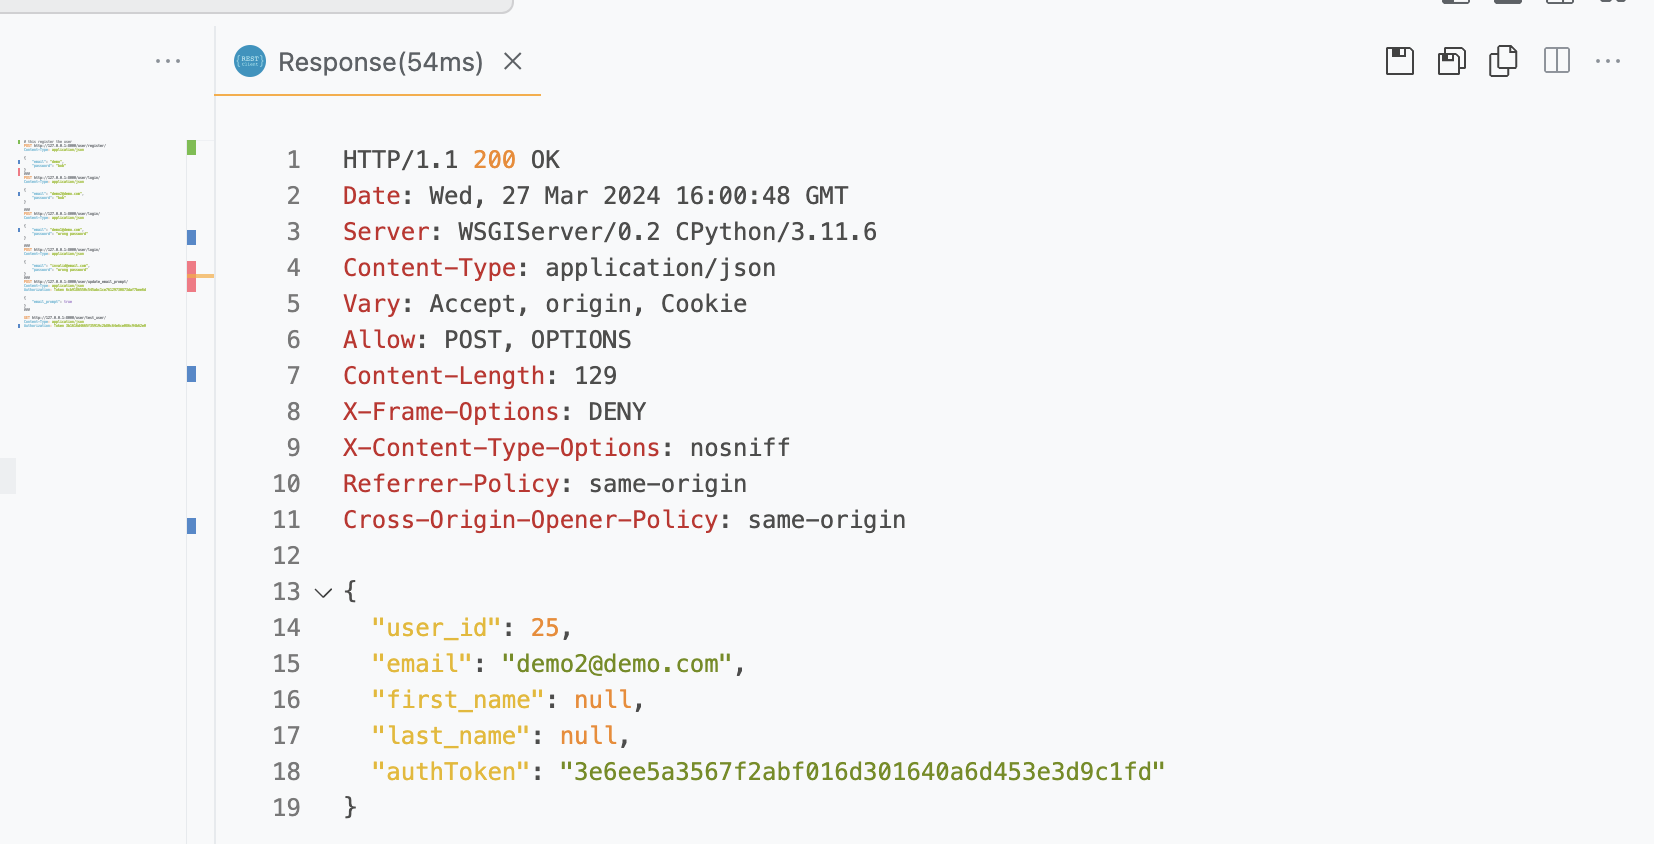
\includegraphics[width=\textwidth]{Assets/api_test/response_login_sucessful.png}
    \label{fig:response_login_sucessful}
\end{figure}

\begin{figure}[H]
    \caption{Request to login with an invalid user}
    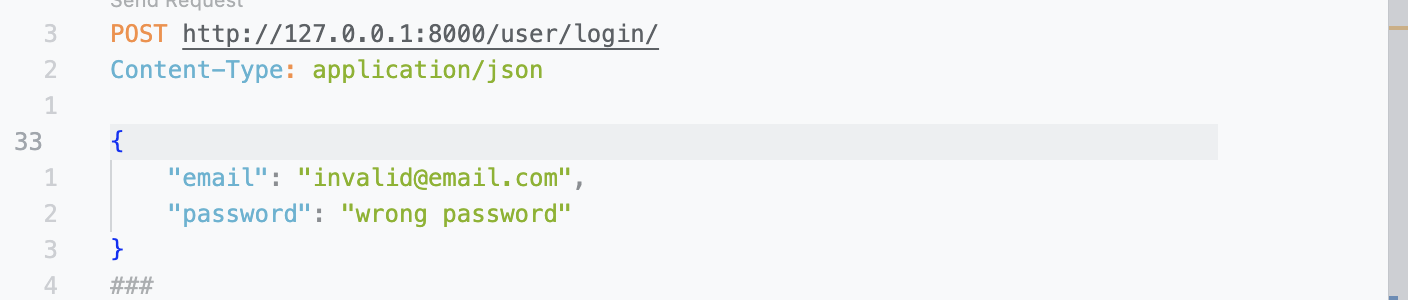
\includegraphics[width=\textwidth]{Assets/api_test/request_login_invalid_user.png}
    \label{fig:request_login_invalid_user}
\end{figure}

\begin{figure}[H]
    \caption{Response to invalid login with an invalid user}
    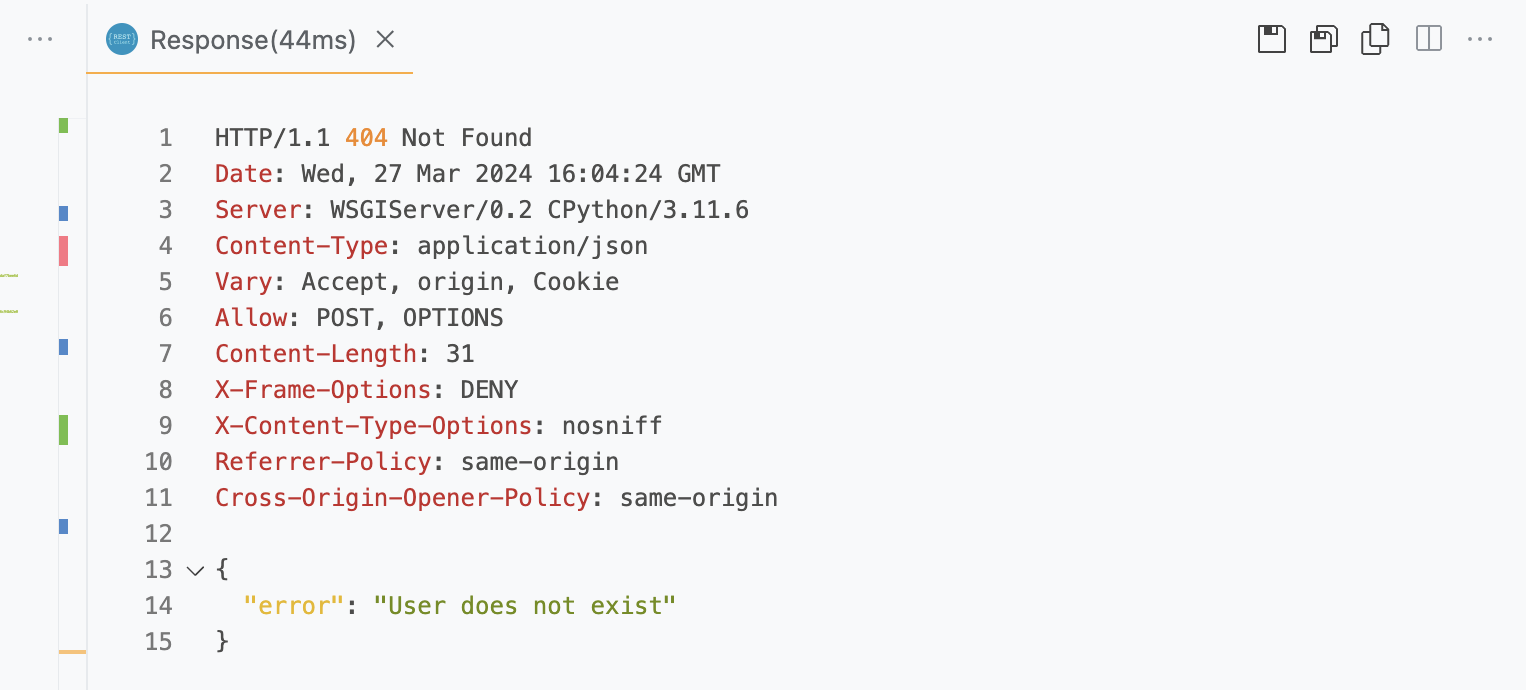
\includegraphics[width=\textwidth]{Assets/api_test/response_login_invalid_user.png}
    \label{fig:response_login_invalid_user}
\end{figure}

\begin{figure}[H]
    \caption{Request to login with an invalid password}
    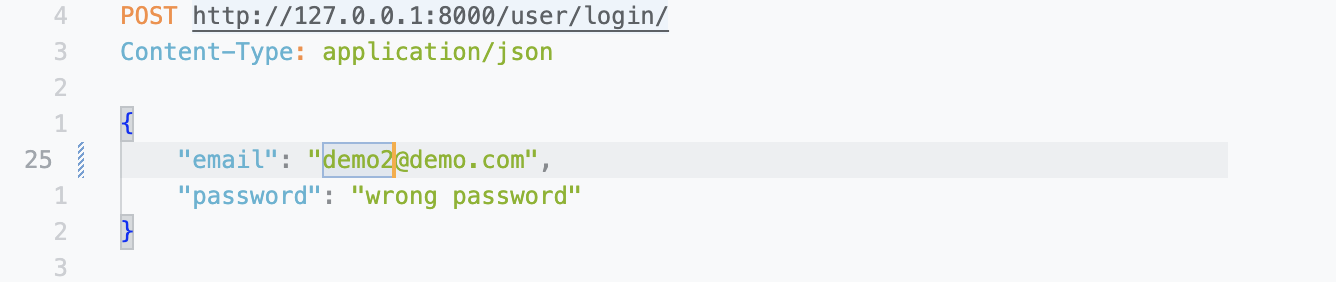
\includegraphics[width=\textwidth]{Assets/api_test/request_login_invalid_password.png}
    \label{fig:request_login_invalid_password}
\end{figure}

\begin{figure}[H]
    \caption{Response to invalid login with an invalid password}
    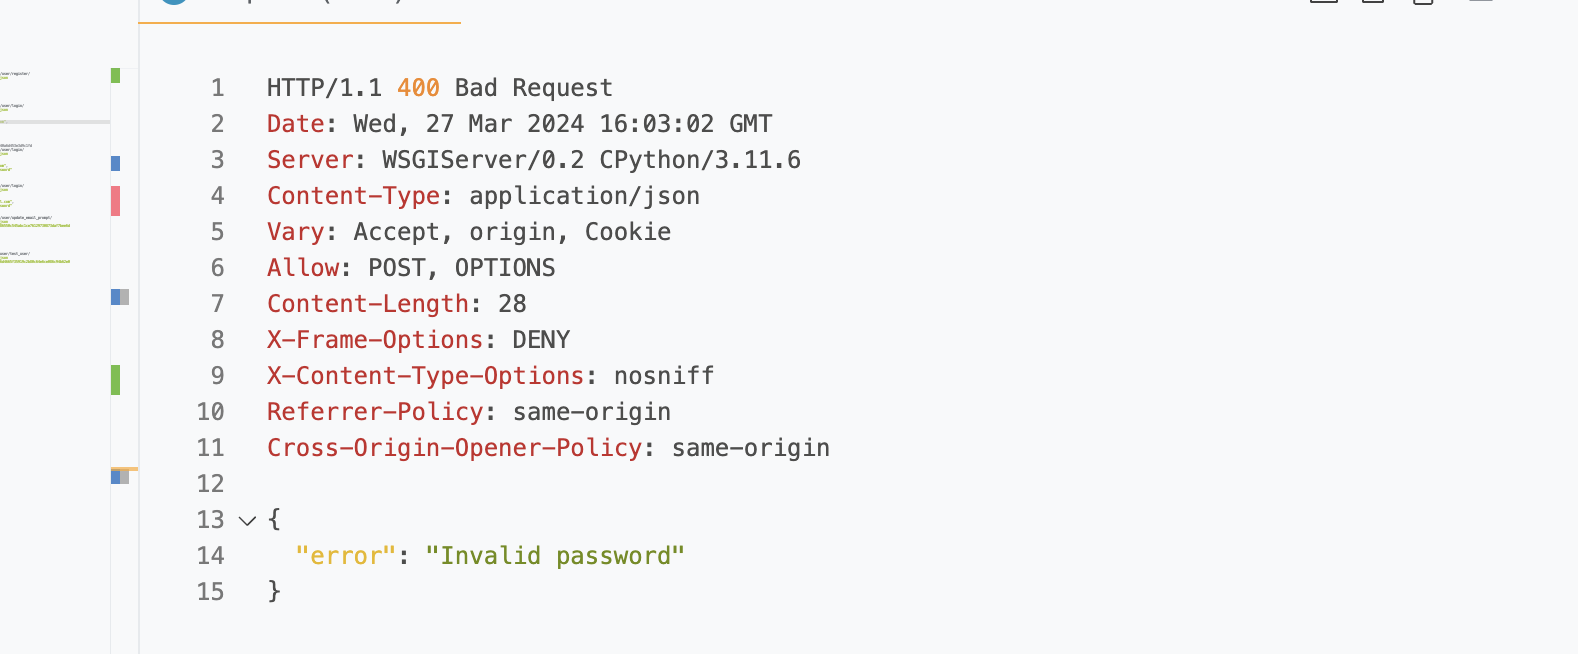
\includegraphics[width=\textwidth]{Assets/api_test/response_login_invalid_password.png}
    \label{fig:response_login_invalid_password}
\end{figure}



\begin{figure}[H]
    \caption{Request to login with an invalid email}
    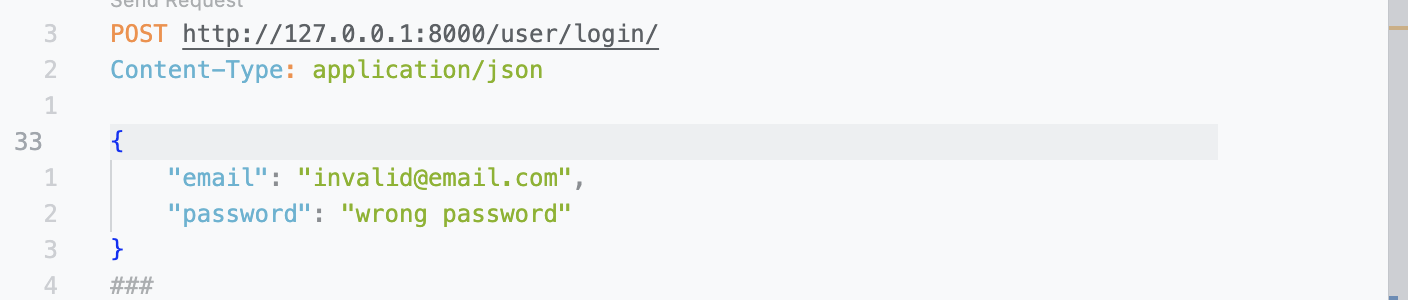
\includegraphics[width=\textwidth]{Assets/api_test/request_login_invalid_user.png}
    \label{fig:request_login_invalid_email}
\end{figure}

\begin{figure}[H]
    \caption{Response to invalid login with an invalid email}
    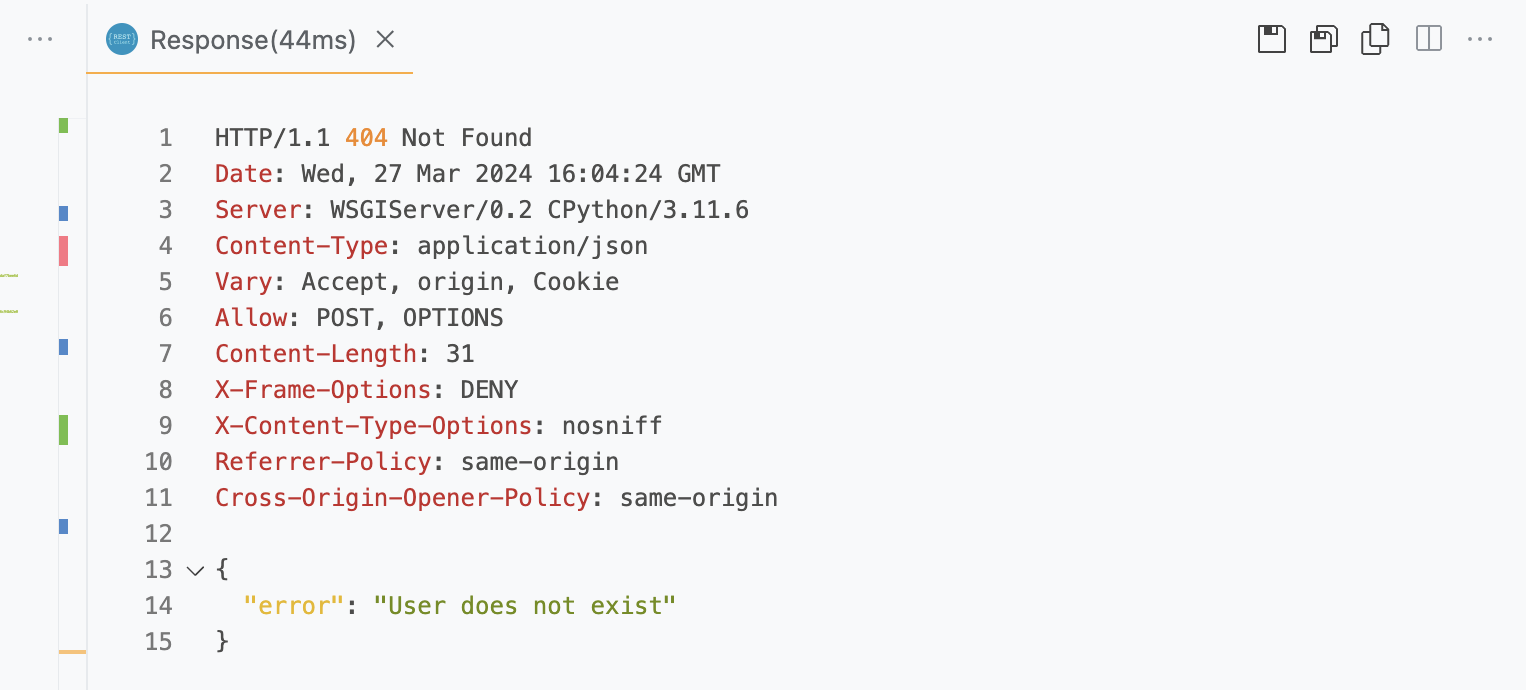
\includegraphics[width=\textwidth]{Assets/api_test/response_login_invalid_user.png}
    \label{fig:response_login_invalid_email}
\end{figure}


\subsection{test\_user/}
This is used to test the user authentication. The user must be authenticated with a token to access this endpoint. Also it tests wether the server is able to retrieve the user information from the token.

\begin{figure}[H]
    \caption{Request to test user authentication with a valid token}
    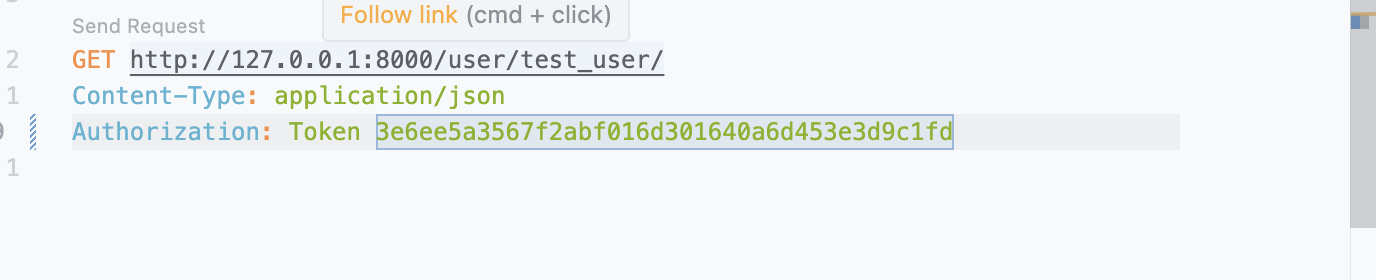
\includegraphics[width=\textwidth]{Assets/api_test/request_test_user_authtoken.png}
    \label{fig:request_test_user_authtoken}
\end{figure}

\begin{figure}[H]
    \caption{Response to test user authentication with a valid token}
    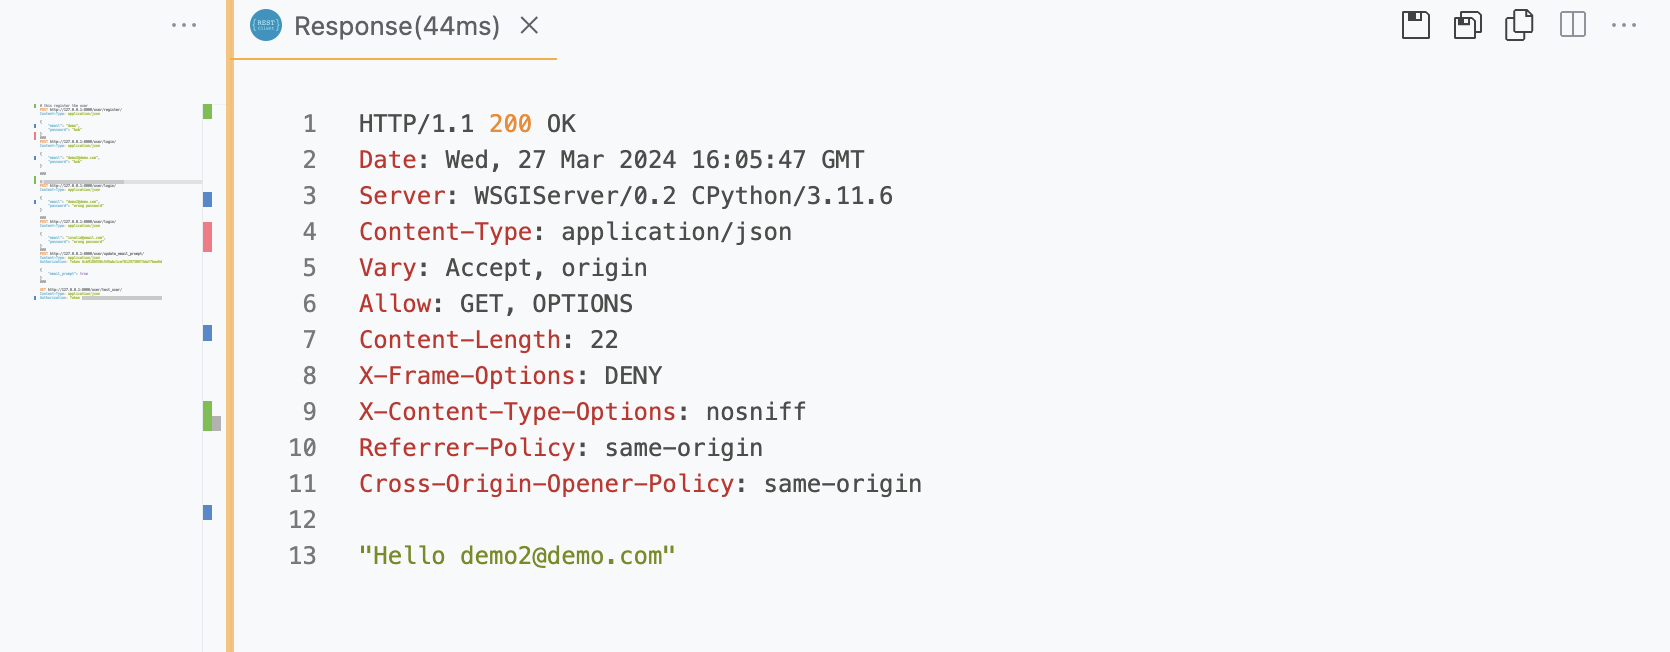
\includegraphics[width=\textwidth]{Assets/api_test/response_test_user_authtoken.png}
    \label{fig:response_test_user_authtoken}
\end{figure}

\begin{figure}[H]
    \caption{Request to test user authentication with an invalid token}
    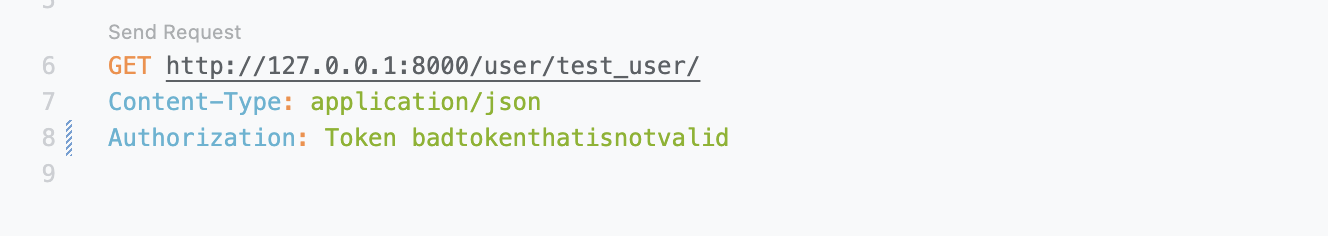
\includegraphics[width=\textwidth]{Assets/api_test/request_test_user_authtoken_invalid.png}
    \label{fig:request_test_user_authtoken_invalid}
\end{figure}

\begin{figure}[H]
    \caption{Response to test user authentication with an invalid token}
    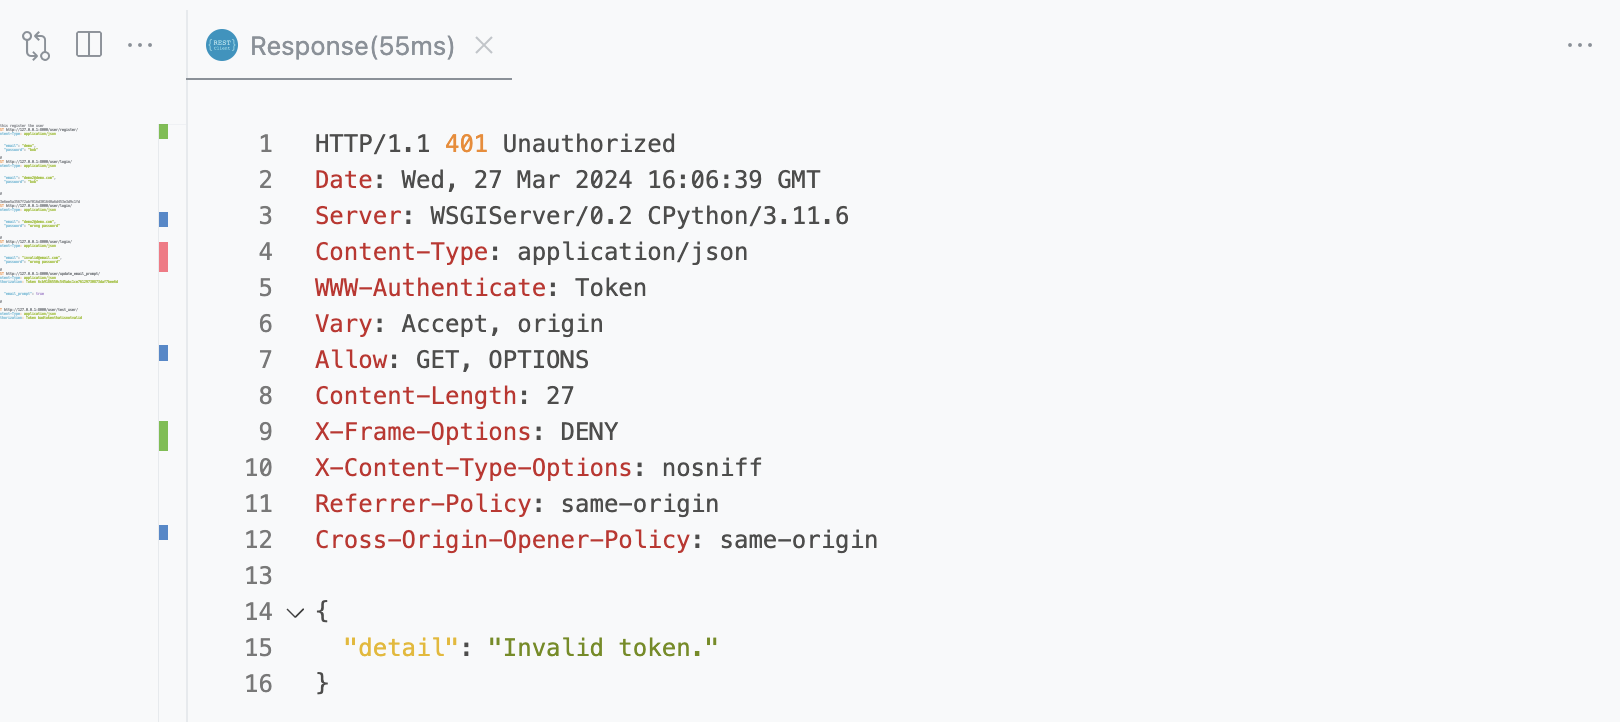
\includegraphics[width=\textwidth]{Assets/api_test/response_test_user_authtoken_invalid.png}
    \label{fig:response_test_user_authtoken_invalid}
\end{figure}

\subsection{Entry App}

\subsection{sample/}
\begin{figure}[H]
    \caption{Request to get samples}
    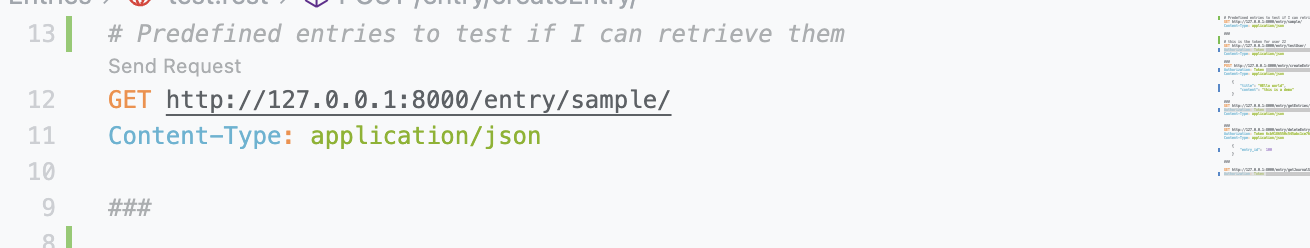
\includegraphics[width=\textwidth]{Assets/api_test/request_get_samples.png}
    \label{fig:request_get_samples}
\end{figure}

\begin{figure}[H]
    \caption{Response to get samples}
    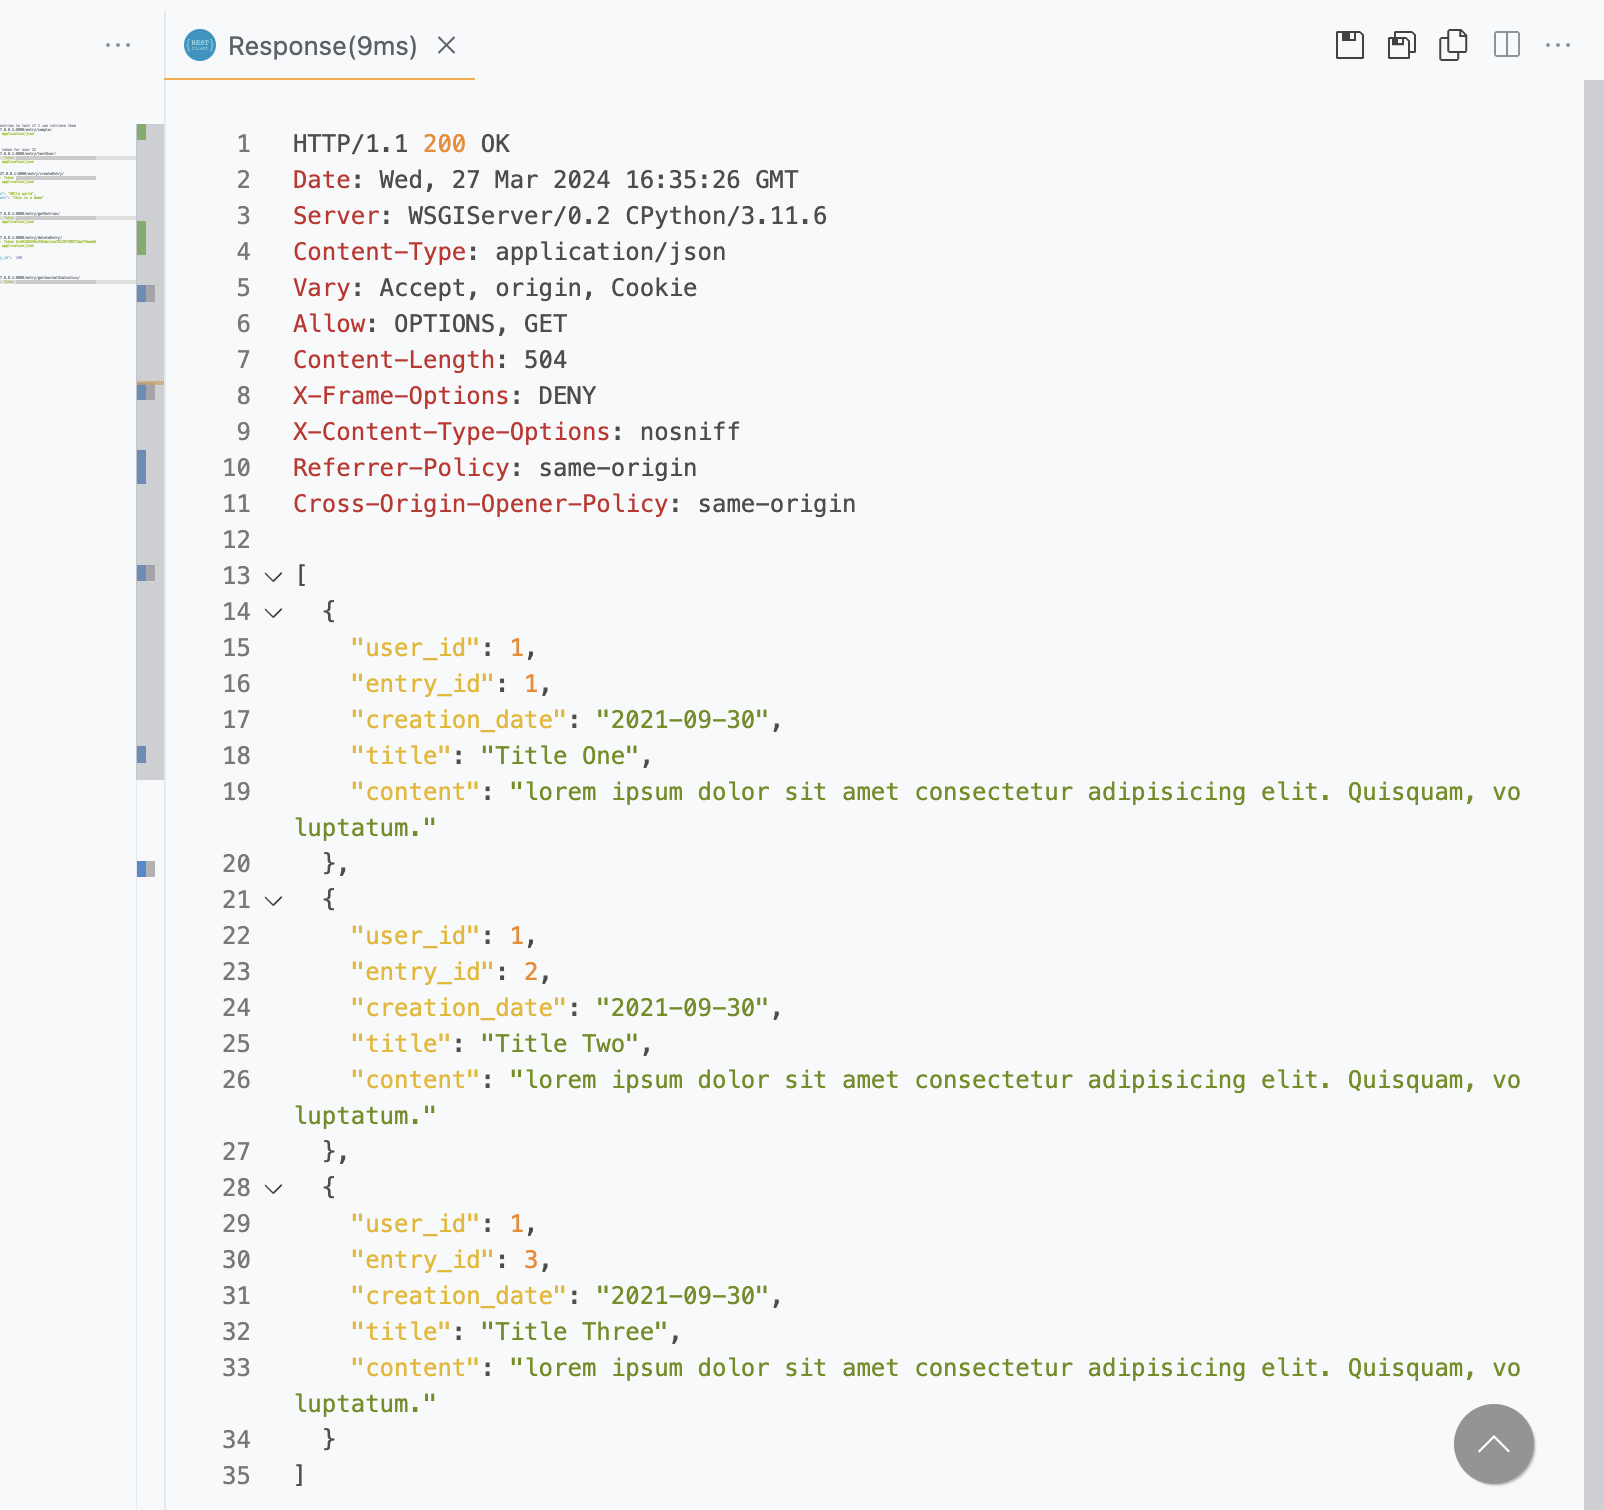
\includegraphics[width=\textwidth]{Assets/api_test/response_get_samples.png}
    \label{fig:response_get_samples}
\end{figure}

\subsection{testUser/}
\begin{figure}[H]
    \caption{Request to test user in entry app}
    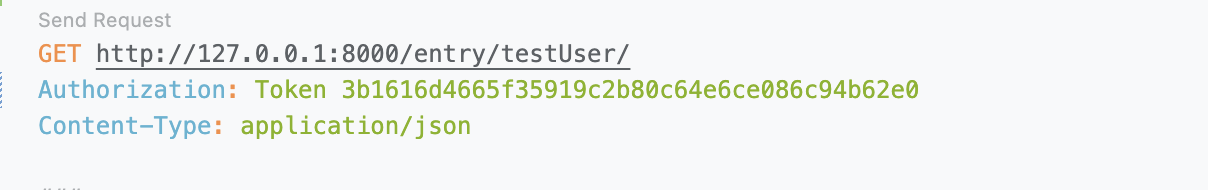
\includegraphics[width=\textwidth]{Assets/api_test/request_test_user_entry.png}
    \label{fig:request_test_user_entry}
\end{figure}

\begin{figure}[H]
    \caption{Response to test user in entry app}
    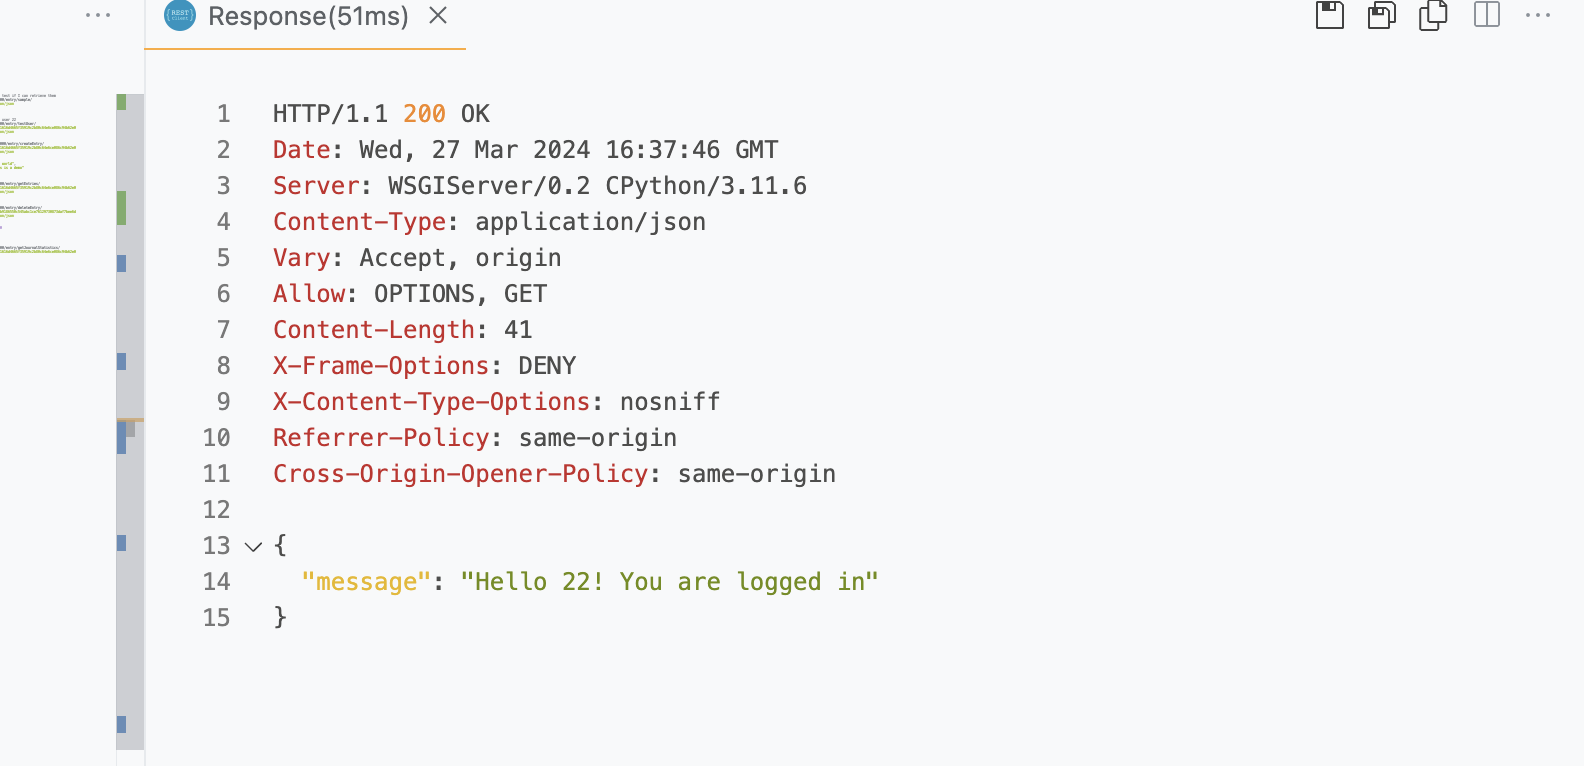
\includegraphics[width=\textwidth]{Assets/api_test/response_test_user_entry.png}
    \label{fig:response_test_user_entry}
\end{figure}

\subsection{createEntry/}
\begin{figure}[H]
    \caption{Request to create a new entry}
    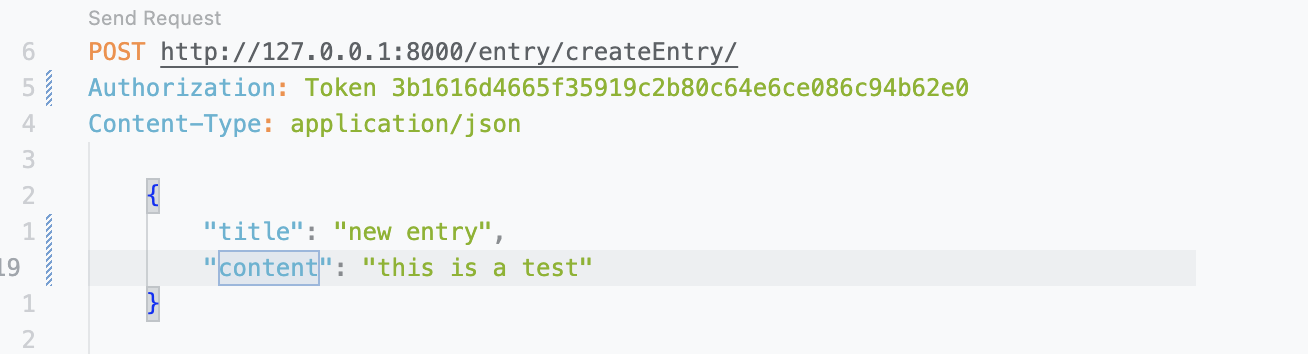
\includegraphics[width=\textwidth]{Assets/api_test/request_create_new_entry.png}
    \label{fig:request_create_new_entry}
\end{figure}

\begin{figure}[H]
    \caption{Response to creating a new entry}
    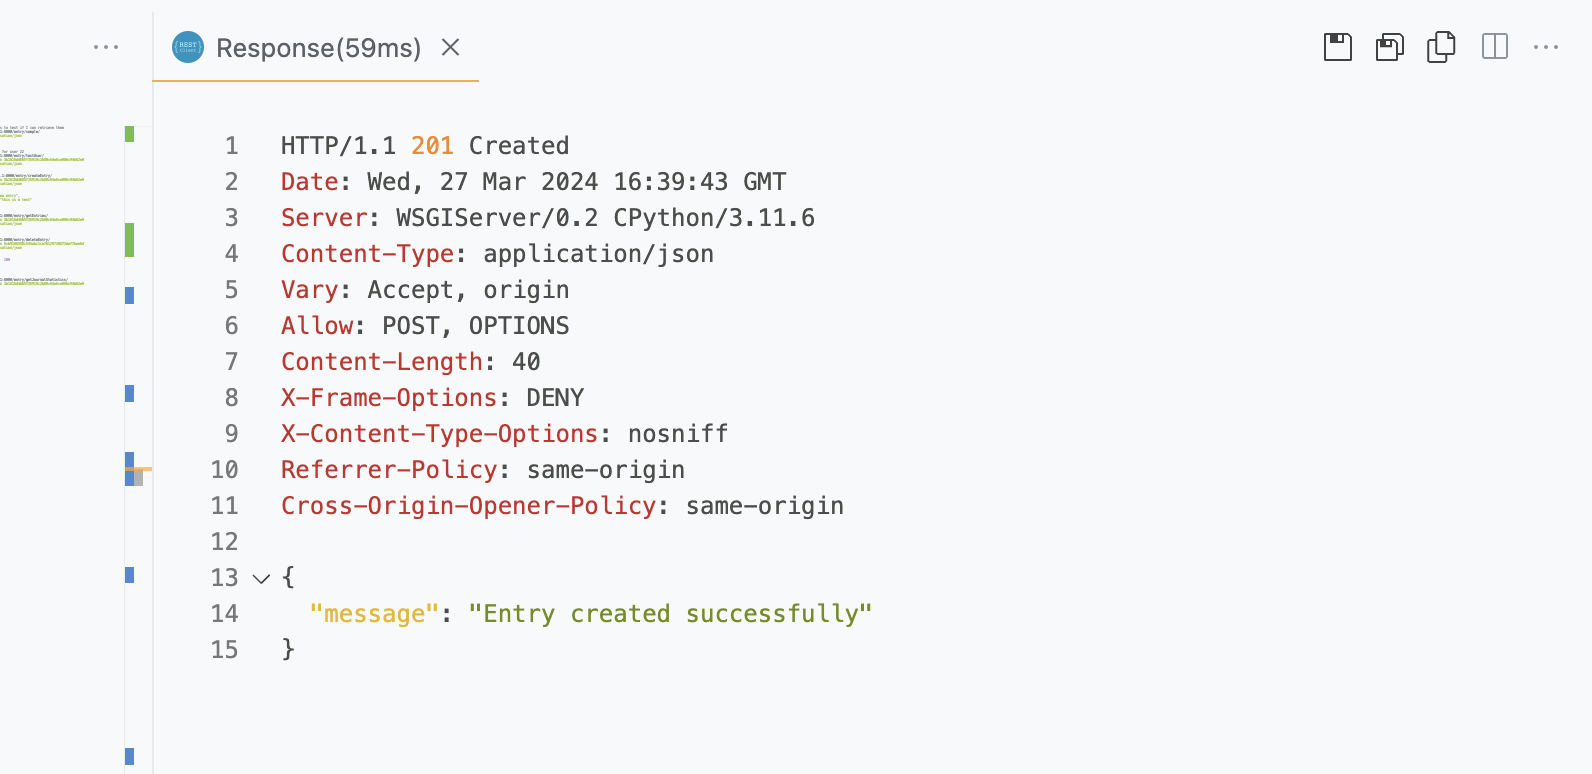
\includegraphics[width=\textwidth]{Assets/api_test/response_create_new_entry.png}
    \label{fig:response_create_new_entry}
\end{figure}

\subsection{getEntries/}
\begin{figure}[H]
    \caption{Request to get an entry}
    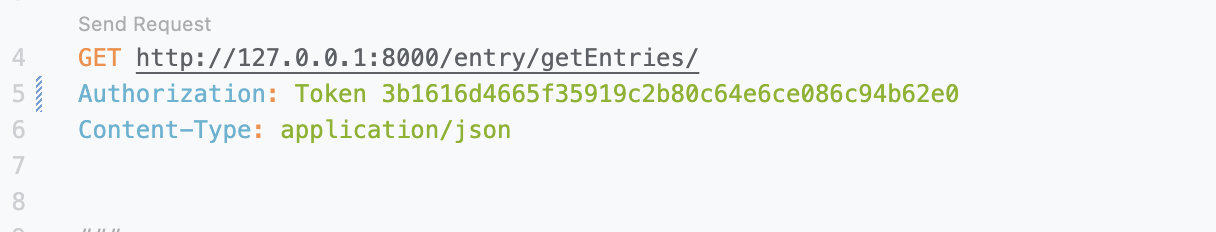
\includegraphics[width=\textwidth]{Assets/api_test/request_get_entry.png}
    \label{fig:request_get_entry}
\end{figure}

\begin{figure}[H]
    \caption{Response to get an entry}
    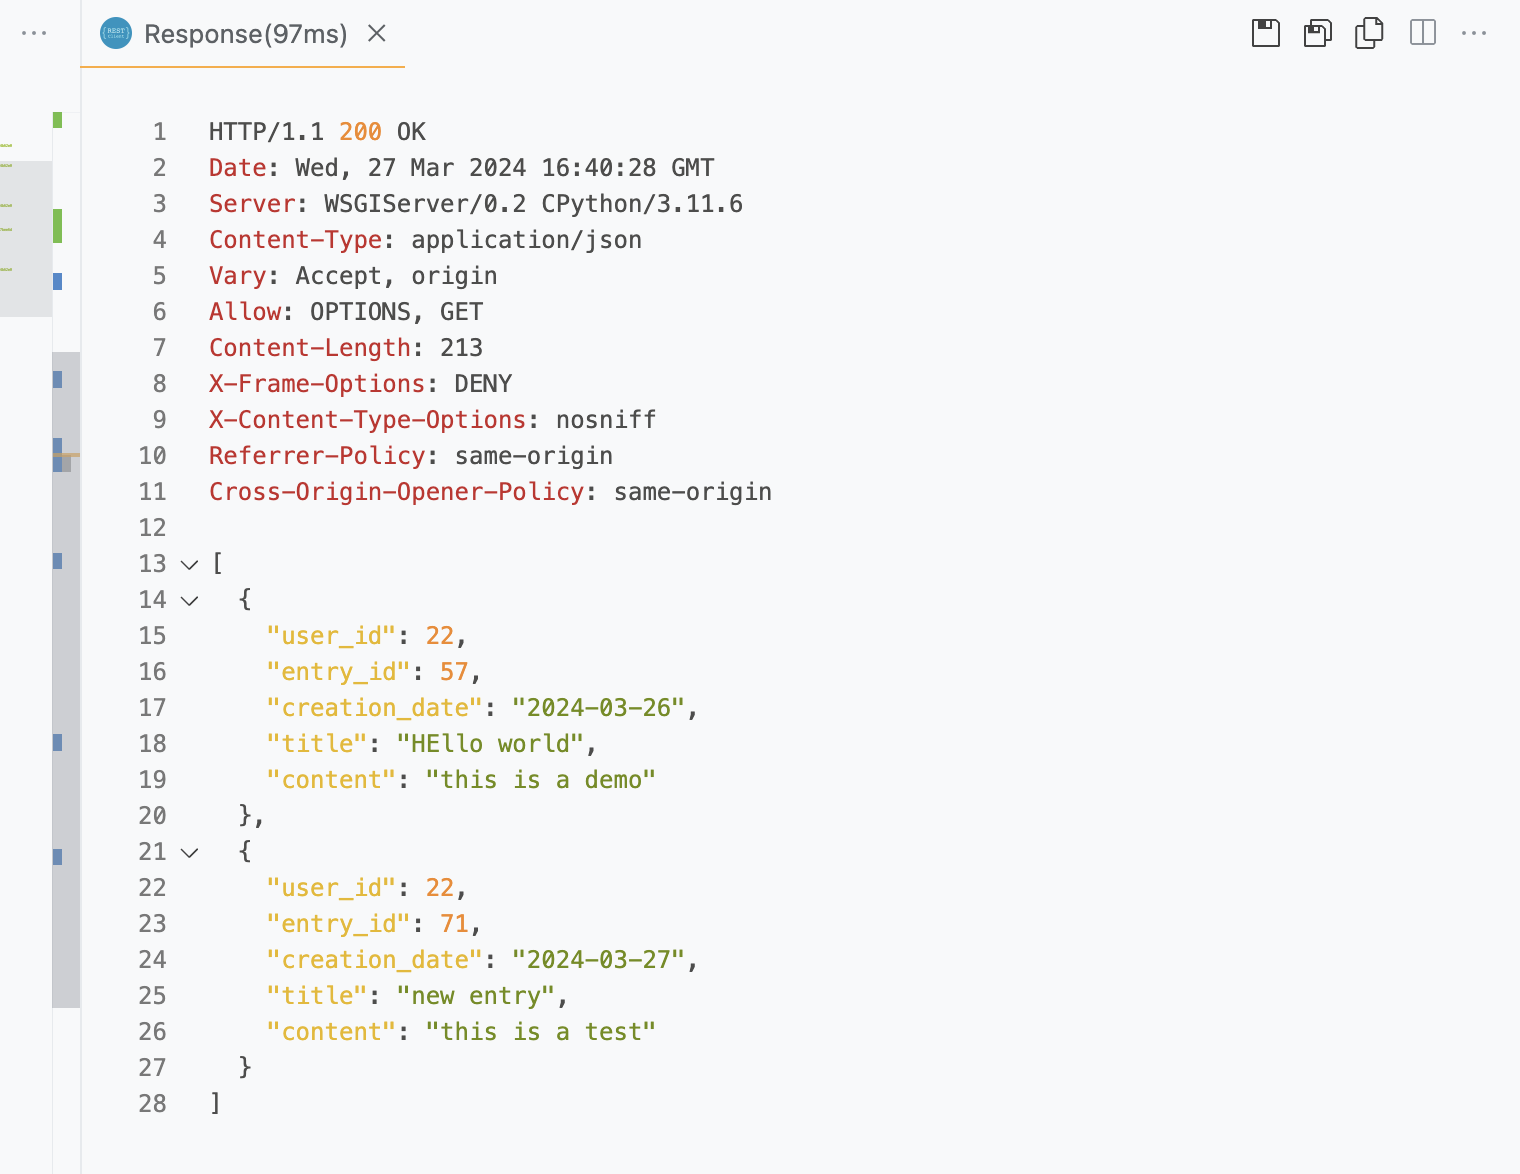
\includegraphics[width=\textwidth]{Assets/api_test/response_get_entry.png}
    \label{fig:response_get_entry}
\end{figure}

\subsection{deleteEntry/}
\begin{figure}[H]
    \caption{Request to delete an entry with an invalid id}
    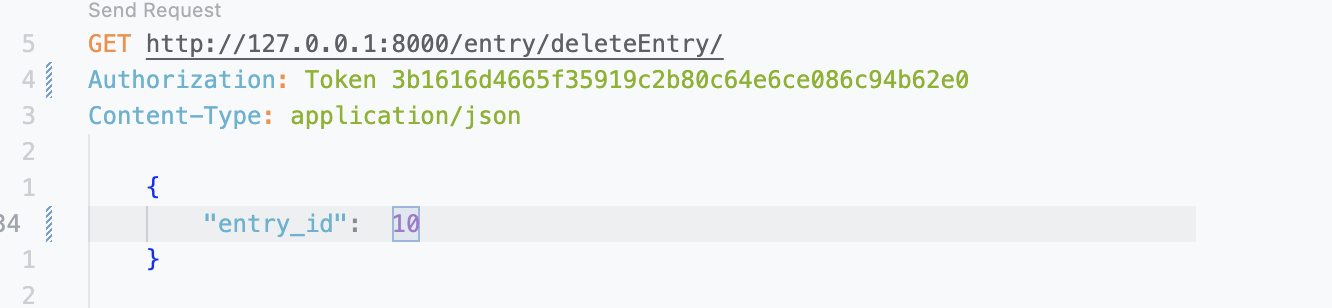
\includegraphics[width=\textwidth]{Assets/api_test/request_delete_entry_invalid.png}
    \label{fig:request_delete_entry_invalid}
\end{figure}

\begin{figure}[H]
    \caption{Response to invalid delete entry request with invalid id}
    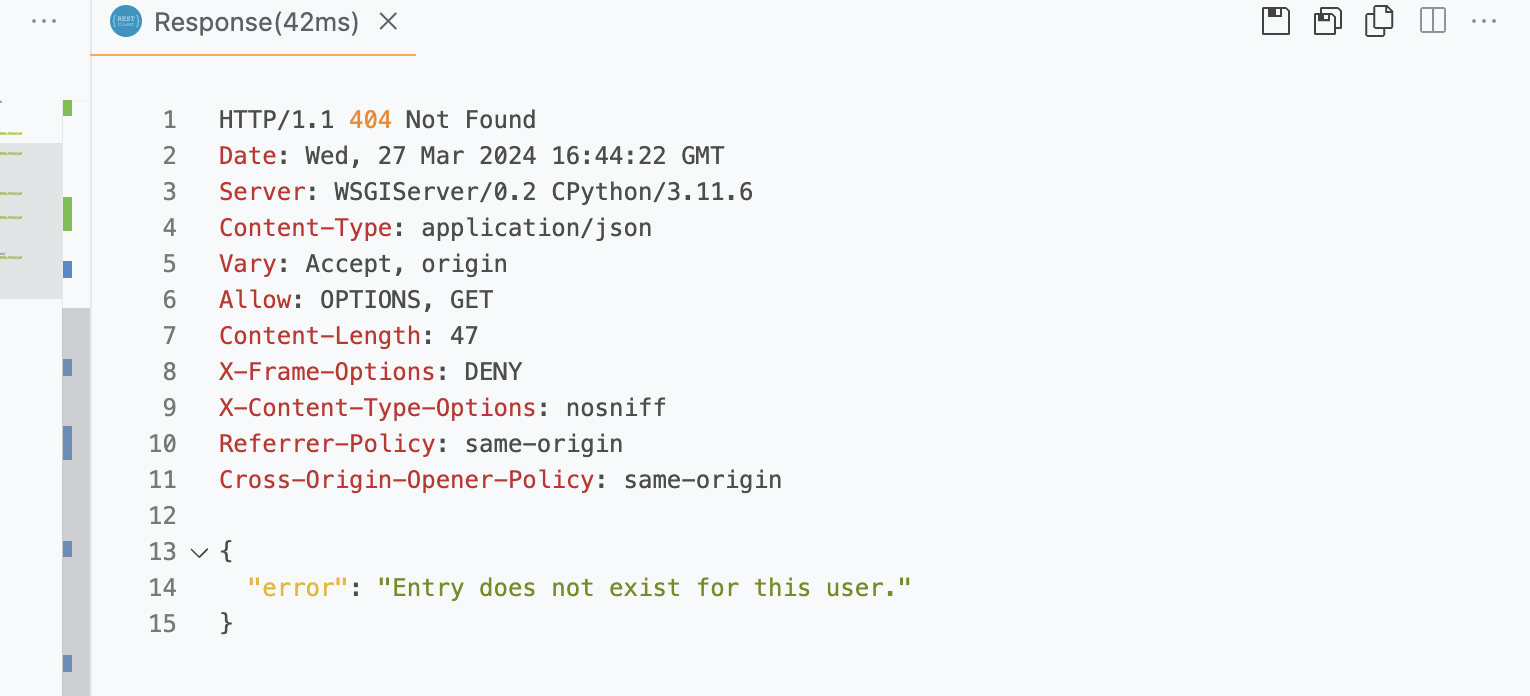
\includegraphics[width=\textwidth]{Assets/api_test/response_delete_entry_invalid.png}
    \label{fig:response_delete_entry_invalid}
\end{figure}

\begin{figure}[H]
    \caption{Request to delete an entry with valid id}
    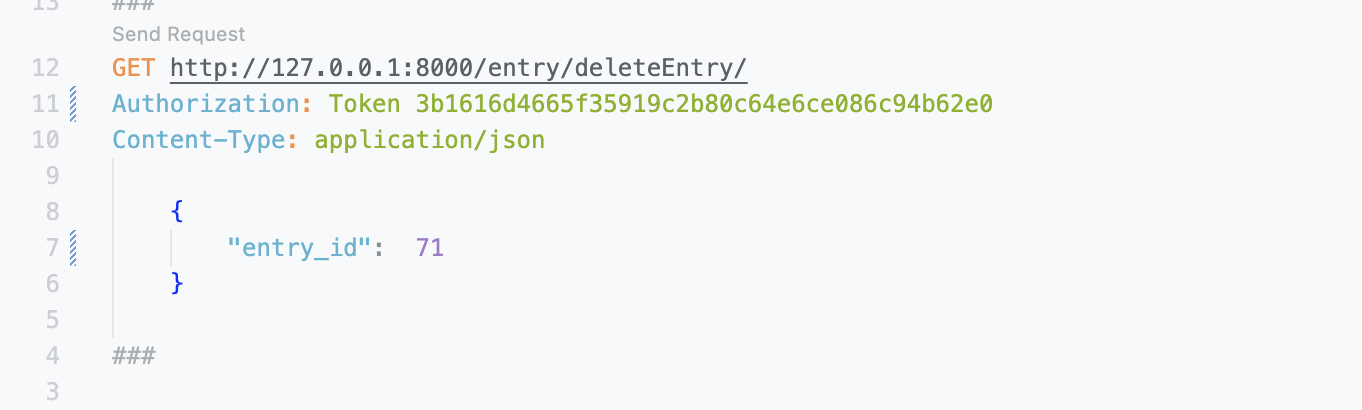
\includegraphics[width=\textwidth]{Assets/api_test/request_delete_entry_valid.png}
    \label{fig:request_delete_entry_valid}
\end{figure}

\begin{figure}[H]
    \caption{Response to valid delete entry request with valid id}
    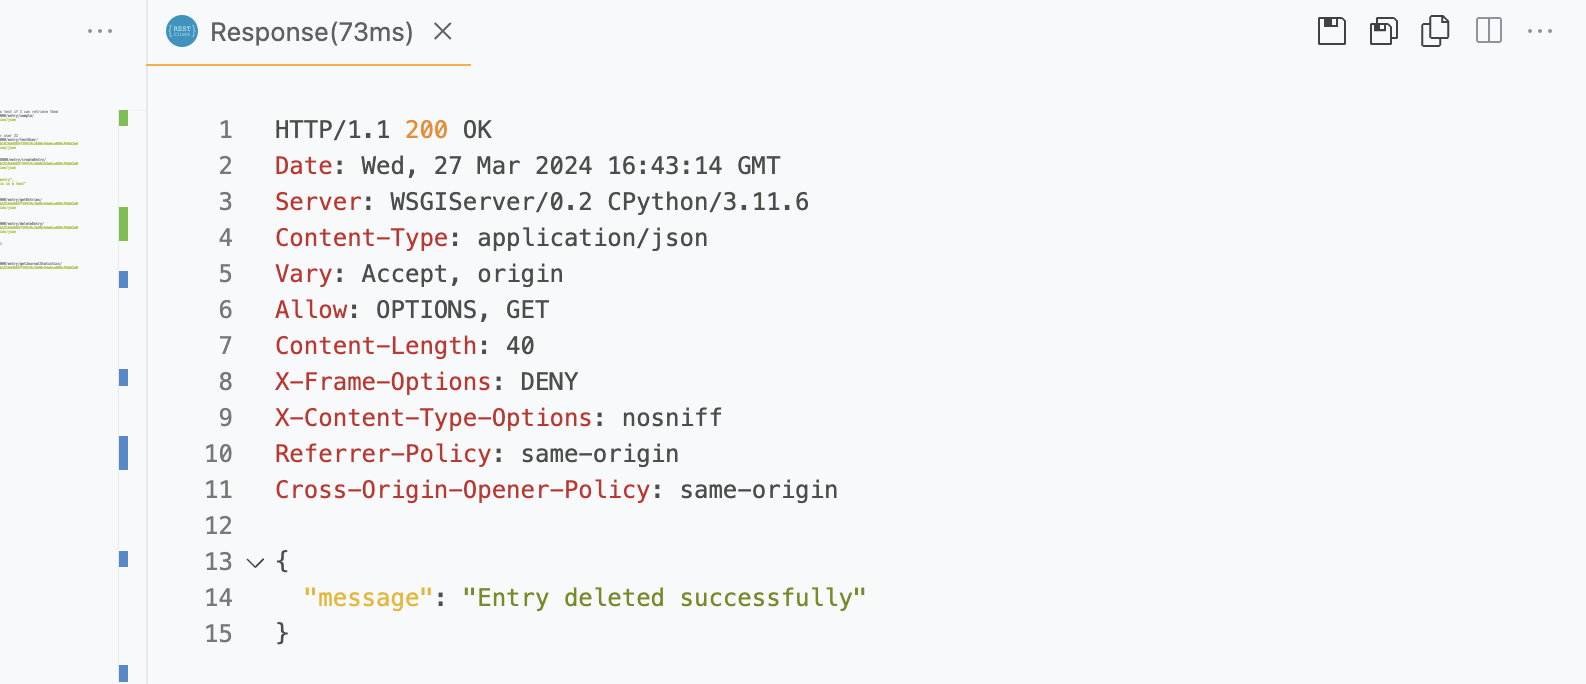
\includegraphics[width=\textwidth]{Assets/api_test/response_delete_entry_valid.png}
    \label{fig:response_delete_entry_valid}
\end{figure}

\subsection{getJournalStatistics/}
\begin{figure}[H]
    \caption{Request to get journal statistics}
    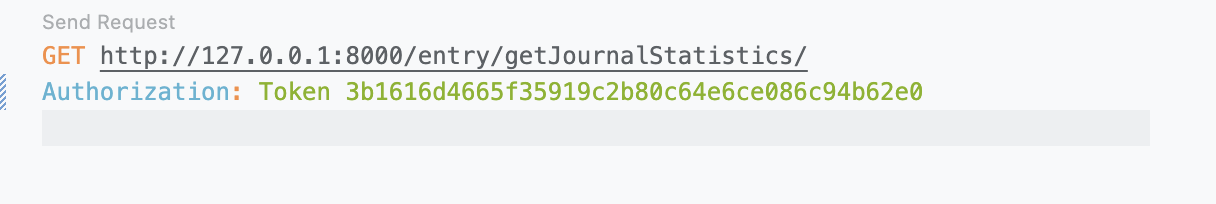
\includegraphics[width=\textwidth]{Assets/api_test/request_get_journal_statistics.png}
    \label{fig:request_get_journal_statistics}
\end{figure}

\begin{figure}[H]
    \caption{Response to get journal statistics}
    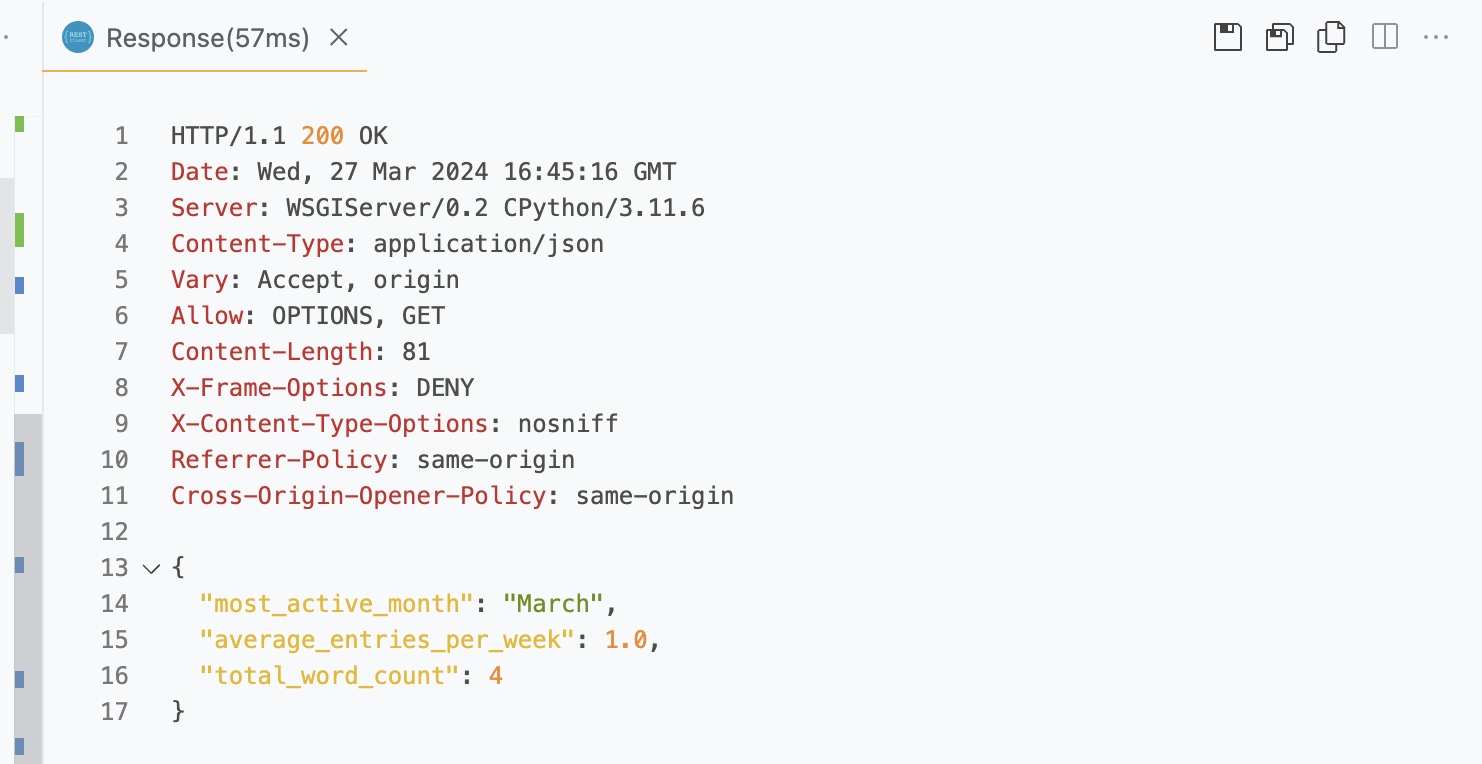
\includegraphics[width=\textwidth]{Assets/api_test/response_get_journal_statistics.png}
    \label{fig:response_get_journal_statistics}
\end{figure}


\section{Git Log}
% use minted to display file
\inputminted{bash}{Assets/git_log.txt}

\section{Code Listings}

\subsubsection{/backend/JournalApp/settings.py}
\inputminted{python3}{SourceCode/backend/JournalApp/settings.py}
\subsubsection{/backend/JournalApp/urls.py}
\inputminted{python3}{SourceCode/backend/JournalApp/urls.py}
\subsubsection{/backend/Users/admin.py}
\inputminted{python3}{SourceCode/backend/Users/admin.py}
\subsubsection{/backend/Users/apps.py}
\inputminted{python3}{SourceCode/backend/Users/apps.py}
\subsubsection{/backend/Users/models.py}
\inputminted{python3}{SourceCode/backend/Users/models.py}
\subsubsection{/backend/Users/serializers.py}
\inputminted{python3}{SourceCode/backend/Users/serializers.py}
\subsubsection{/backend/Users/signals.py}
\inputminted{python3}{SourceCode/backend/Users/signals.py}
\subsubsection{/backend/Users/urls.py}
\inputminted{python3}{SourceCode/backend/Users/urls.py}
\subsubsection{/backend/Users/utils.py}
\inputminted{python3}{SourceCode/backend/Users/utils.py}
\subsubsection{/backend/Users/views.py}
\inputminted{python3}{SourceCode/backend/Users/views.py}

\subsubsection{/backend/Entries/admin.py}
\inputminted{python3}{SourceCode/backend/Entries/admin.py}
\subsubsection{/backend/Entries/apps.py}
\inputminted{python3}{SourceCode/backend/Entries/apps.py}
\subsubsection{/backend/Entries/models.py}
\inputminted{python3}{SourceCode/backend/Entries/models.py}
\subsubsection{/backend/Entries/urls.py}
\inputminted{python3}{SourceCode/backend/Entries/urls.py}
\subsubsection{/backend/Entries/views.py}
\inputminted{python3}{SourceCode/backend/Entries/views.py}



\subsubsection{/frontend/src/main.tsx}
\inputminted{typescript}{SourceCode/frontend/src/main.tsx}
\subsubsection{/frontend/src/App.tsx}
\inputminted{typescript}{SourceCode/frontend/src/App.tsx}
\subsubsection{/frontend/src/componets/layout/NavBar.tsx}
\inputminted{typescript}{SourceCode/frontend/src/components/layout/NavBar.tsx}
\subsubsection{/frontend/src/context/userContext.tsx}
\inputminted{typescript}{SourceCode/frontend/src/context/userContext.tsx}
\subsubsection{/frontend/src/hooks/useAuth.ts}
\inputminted{typescript}{SourceCode/frontend/src/hooks/useAuth.ts}
\subsubsection{/frontend/src/hooks/useFetchData.tsx}
\inputminted{typescript}{SourceCode/frontend/src/hooks/useFetchData.tsx}
\subsubsection{/frontend/src/hooks/useUser.ts}
\inputminted{typescript}{SourceCode/frontend/src/hooks/useUser.ts}
\subsubsection{/frontend/src/hooks/useUserContext.ts}
\inputminted{typescript}{SourceCode/frontend/src/hooks/useUserContext.ts}

\subsubsection{/frontend/src/pages/HomePage.tsx}
\inputminted{typescript}{SourceCode/frontend/src/pages/HomePage.tsx}
\subsubsection{/frontend/src/pages/ProfilePage.tsx}
\inputminted{typescript}{SourceCode/frontend/src/pages/ProfilePage.tsx}
\subsubsection{/frontend/src/pages/entry/CreateEntryPage.tsx}
\inputminted{typescript}{SourceCode/frontend/src/pages/entry/CreateEntryPage.tsx}
\subsubsection{/frontend/src/pages/entry/JournalEntiesyPage.tsx}
\inputminted{typescript}{SourceCode/frontend/src/pages/entry/JournalEntriesPage.tsx}
\subsubsection{/frontend/src/pages/entry/sortEntries.ts}
\inputminted{typescript}{SourceCode/frontend/src/pages/entry/sortEntries.ts}
\subsubsection{/frontend/src/pages/login/LoginPage.tsx}
\inputminted{typescript}{SourceCode/frontend/src/pages/login/LoginPage.tsx}
\subsubsection{/frontend/src/pages/register/RegisterPage.tsx}
\inputminted{typescript}{SourceCode/frontend/src/pages/register/RegisterPage.tsx}
\subsubsection{SourceCode/frontend/src/pages/statistics/StatisticsPage.tsx}
\inputminted{typescript}{SourceCode/frontend/src/pages/statistics/StatisticsPage.tsx}








\section{PG Admin Screenshots}
\begin{figure}
    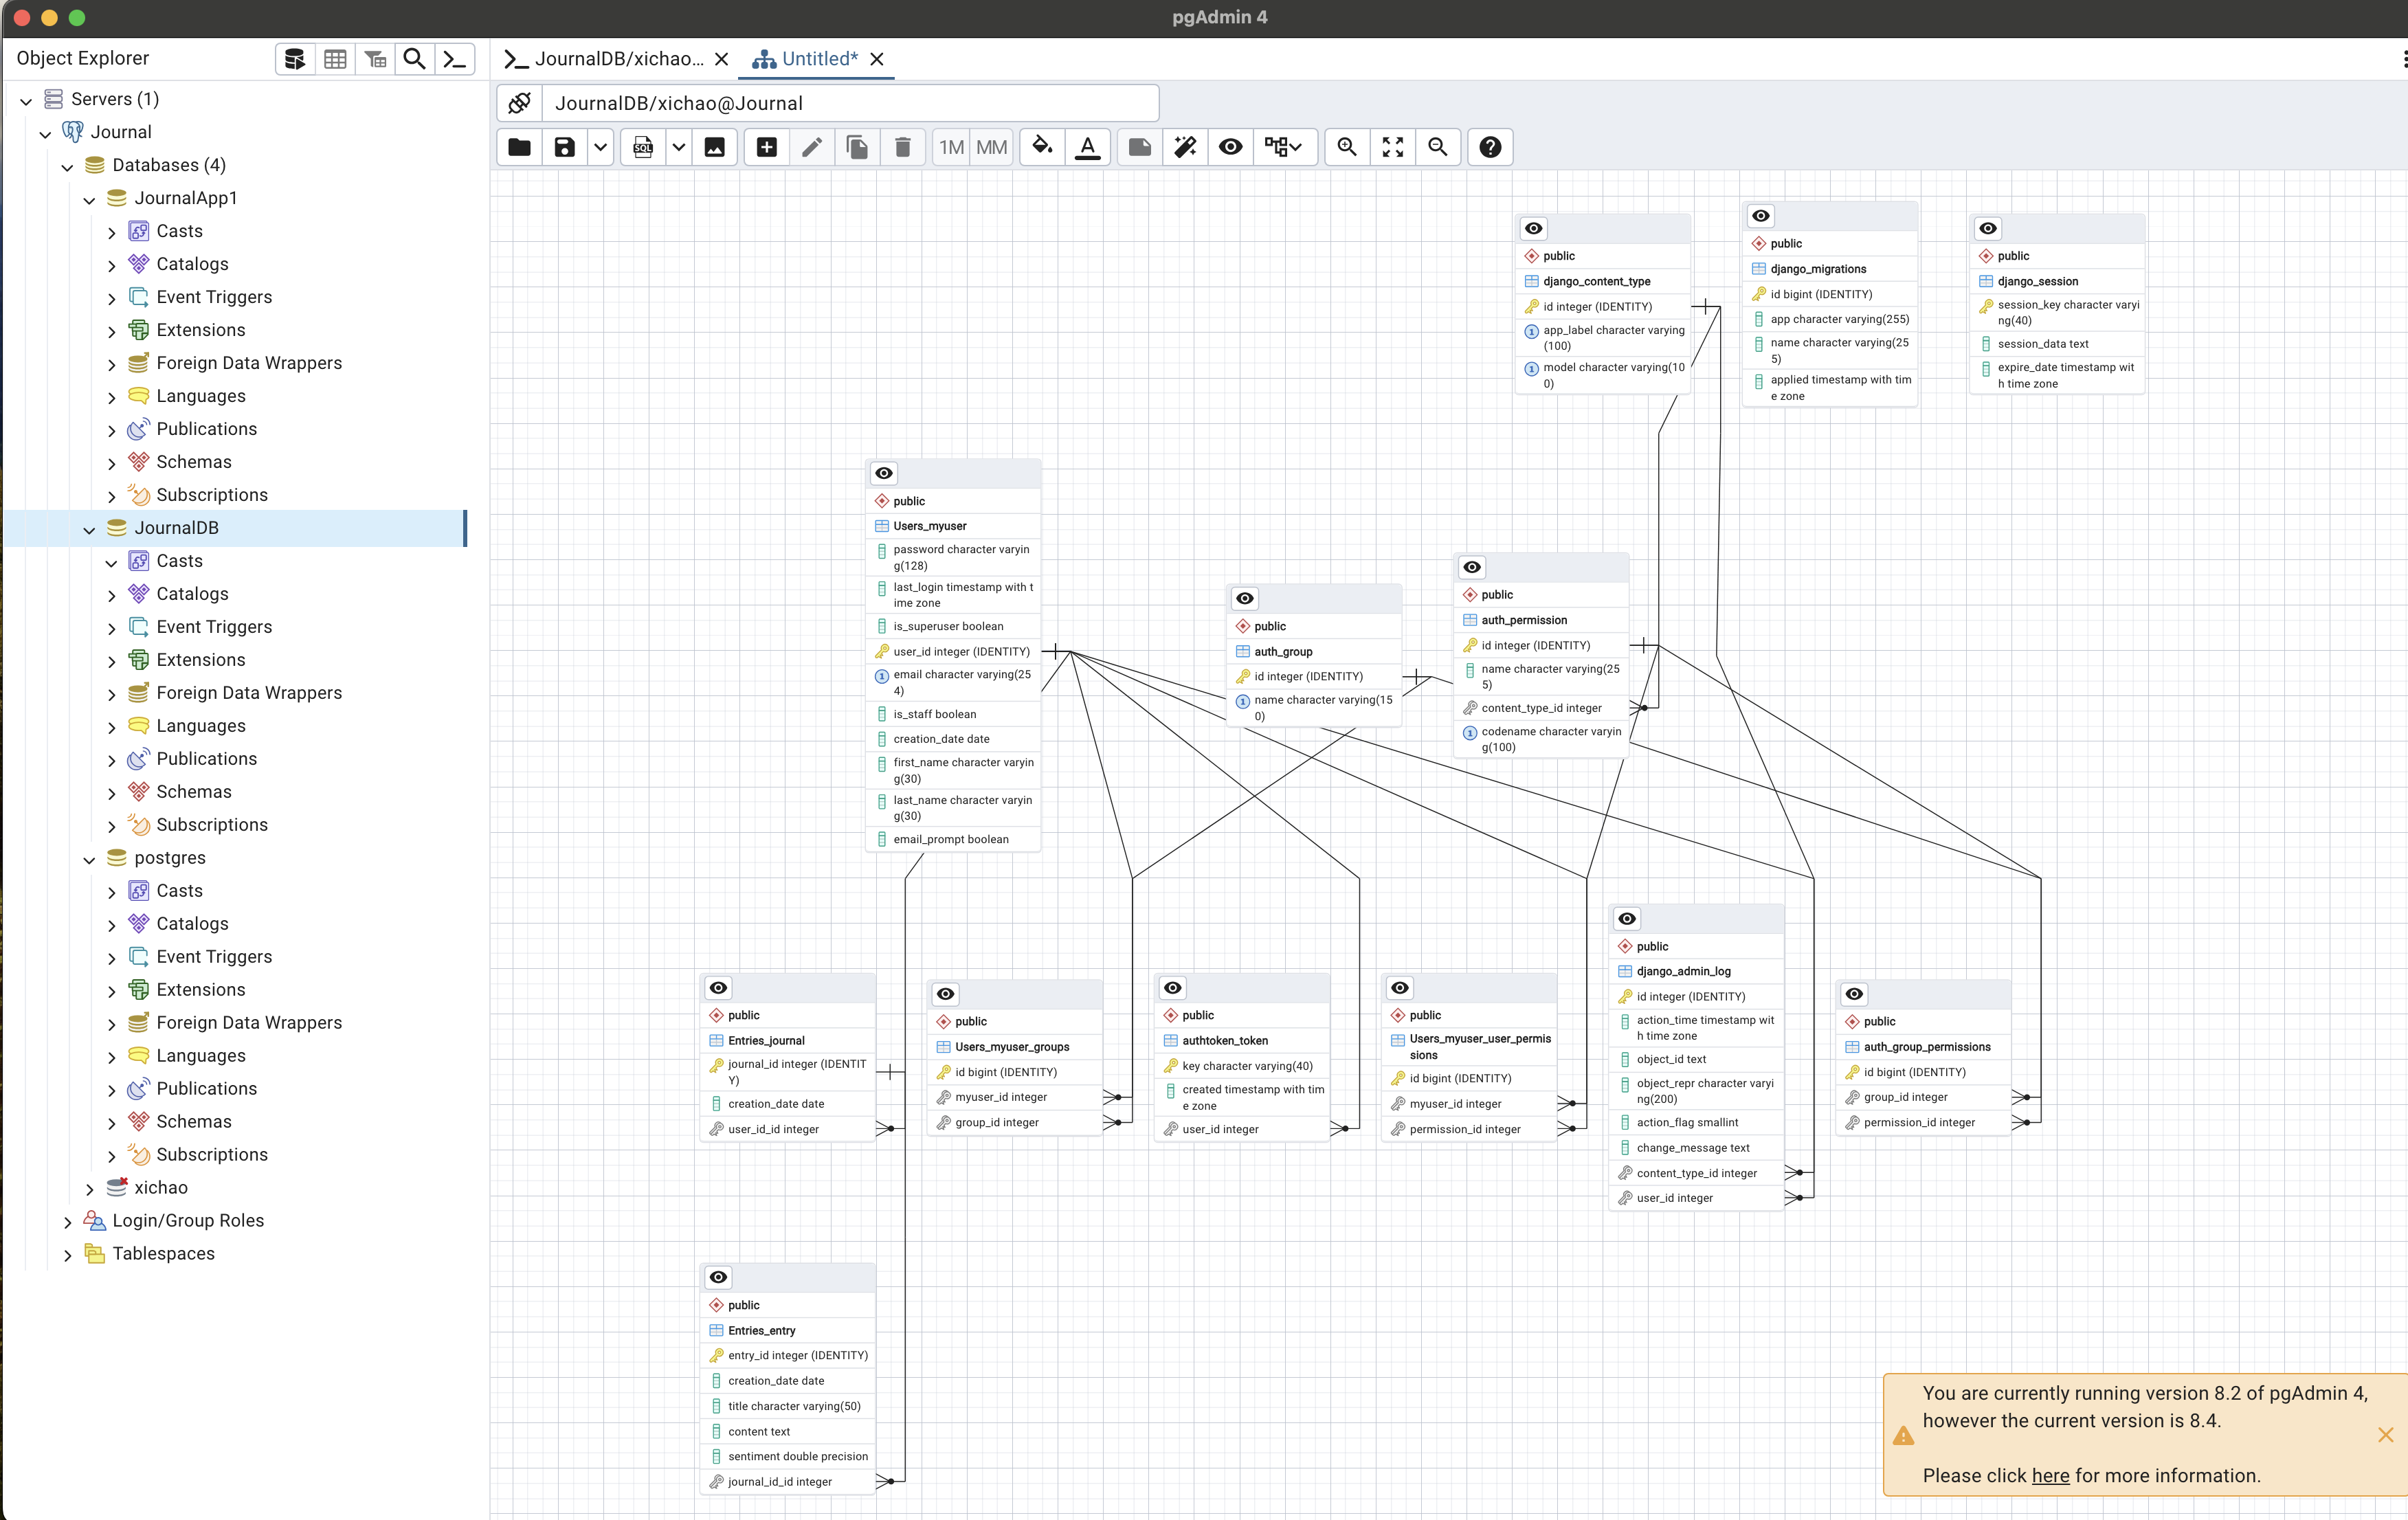
\includegraphics[width=\textwidth]{Assets/pgERD.png}
    \caption{Entity Relation Diagram of the database generated by PG Admin.}
    \label{fig:pgERD}
\end{figure}

\begin{figure}
    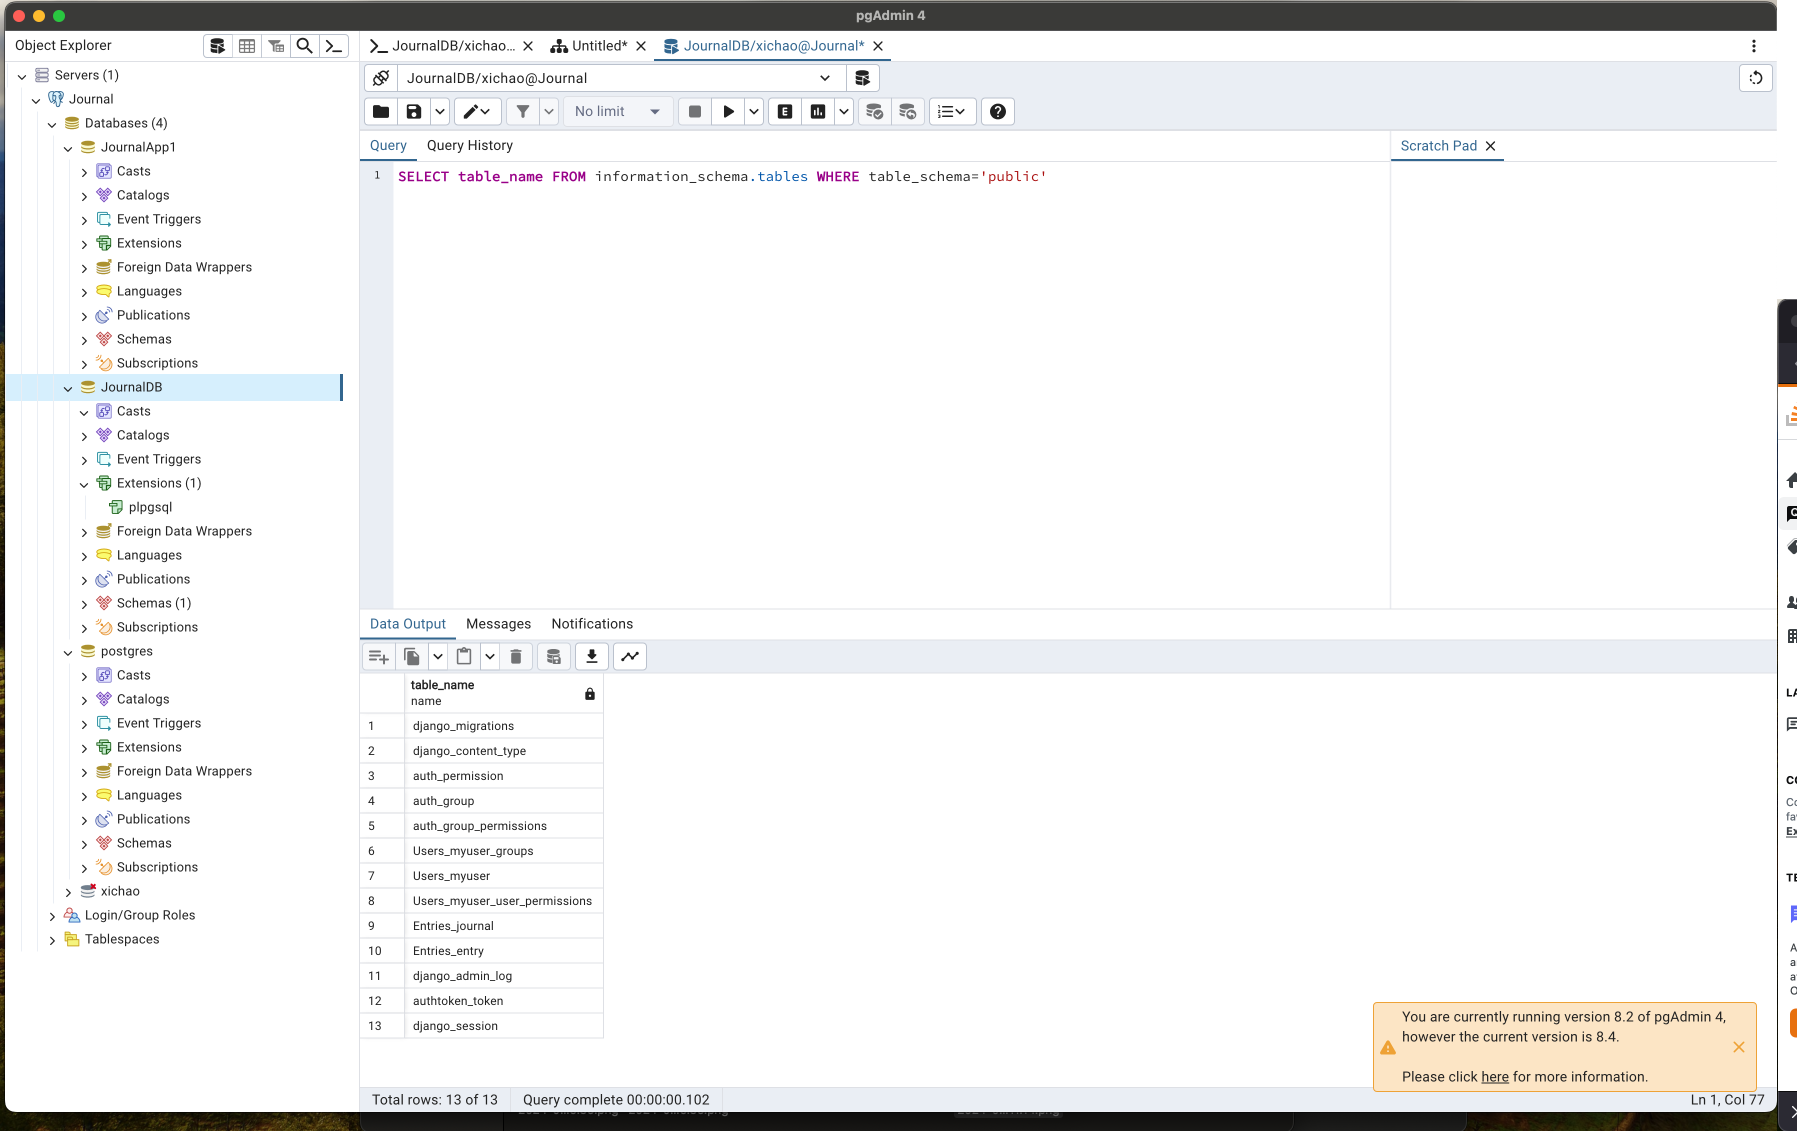
\includegraphics[width=\textwidth]{Assets/pg_all_tables.png}
    \caption{All tables in the database.}
    \label{fig:pg_all_tables}
\end{figure}

\begin{figure}
    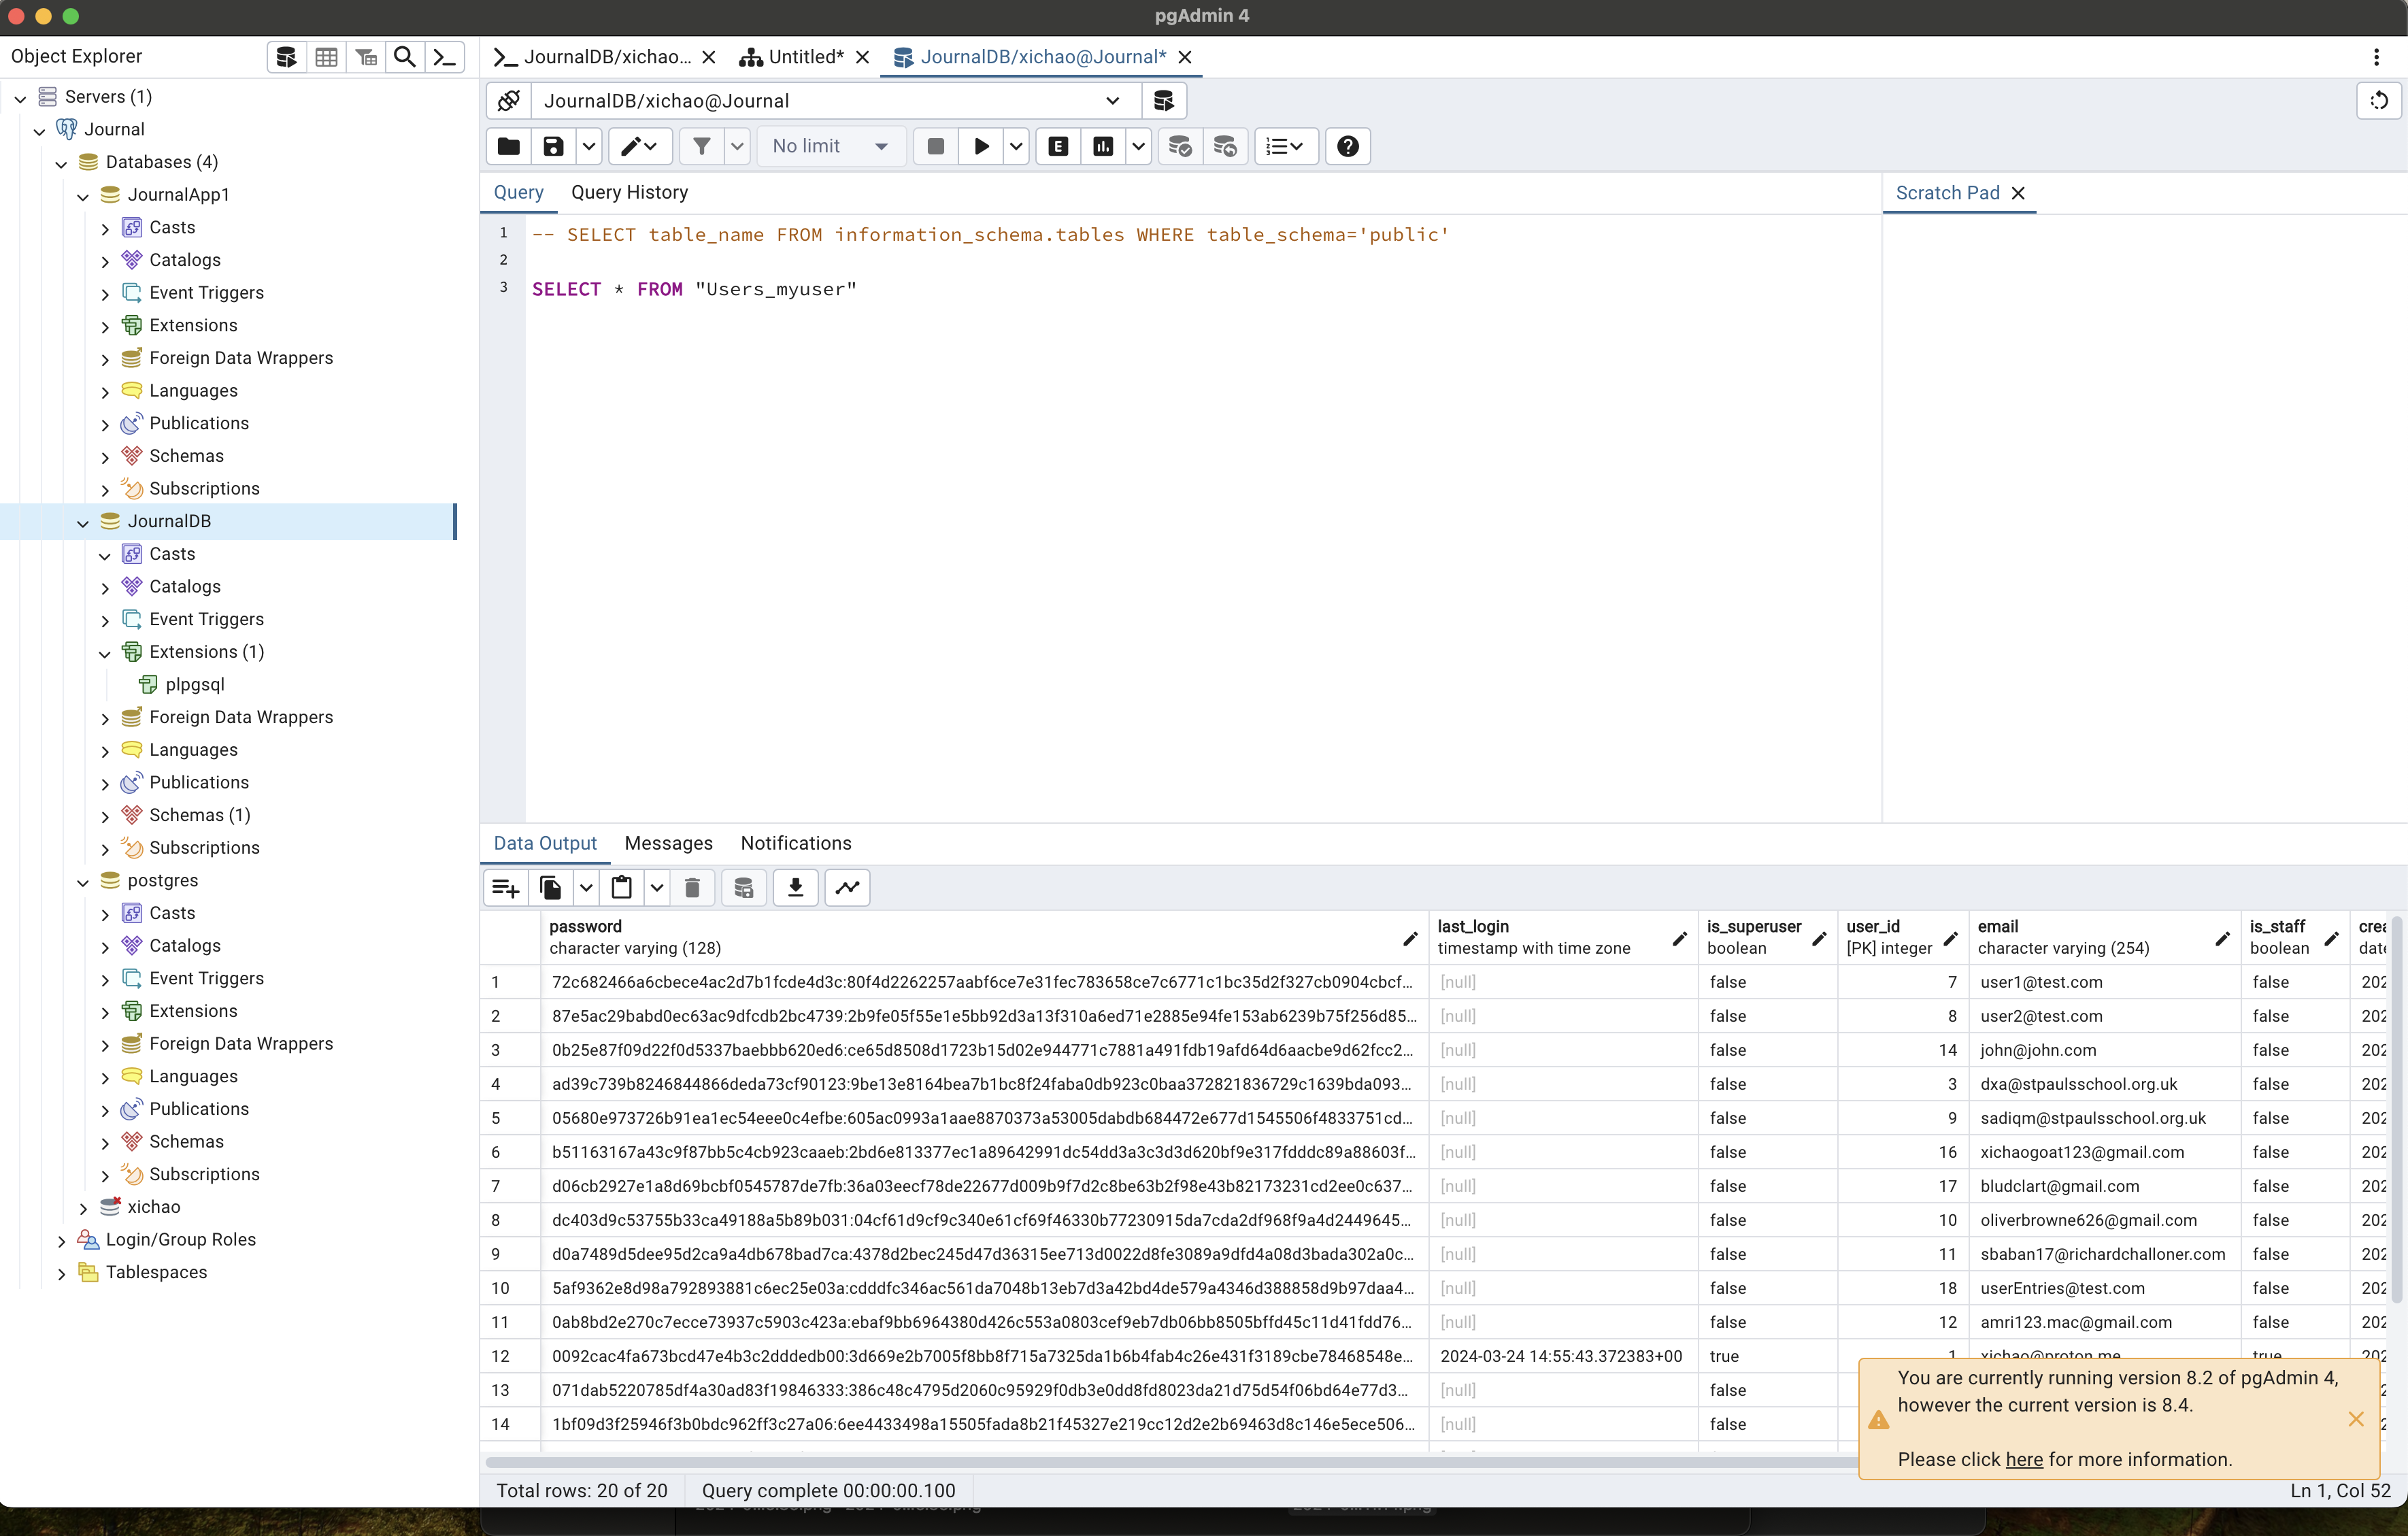
\includegraphics[width=\textwidth]{Assets/pgUsers.png}
    \caption{Users table in the database.}
    \label{fig:pg_users_table}
\end{figure}



\begin{figure}
    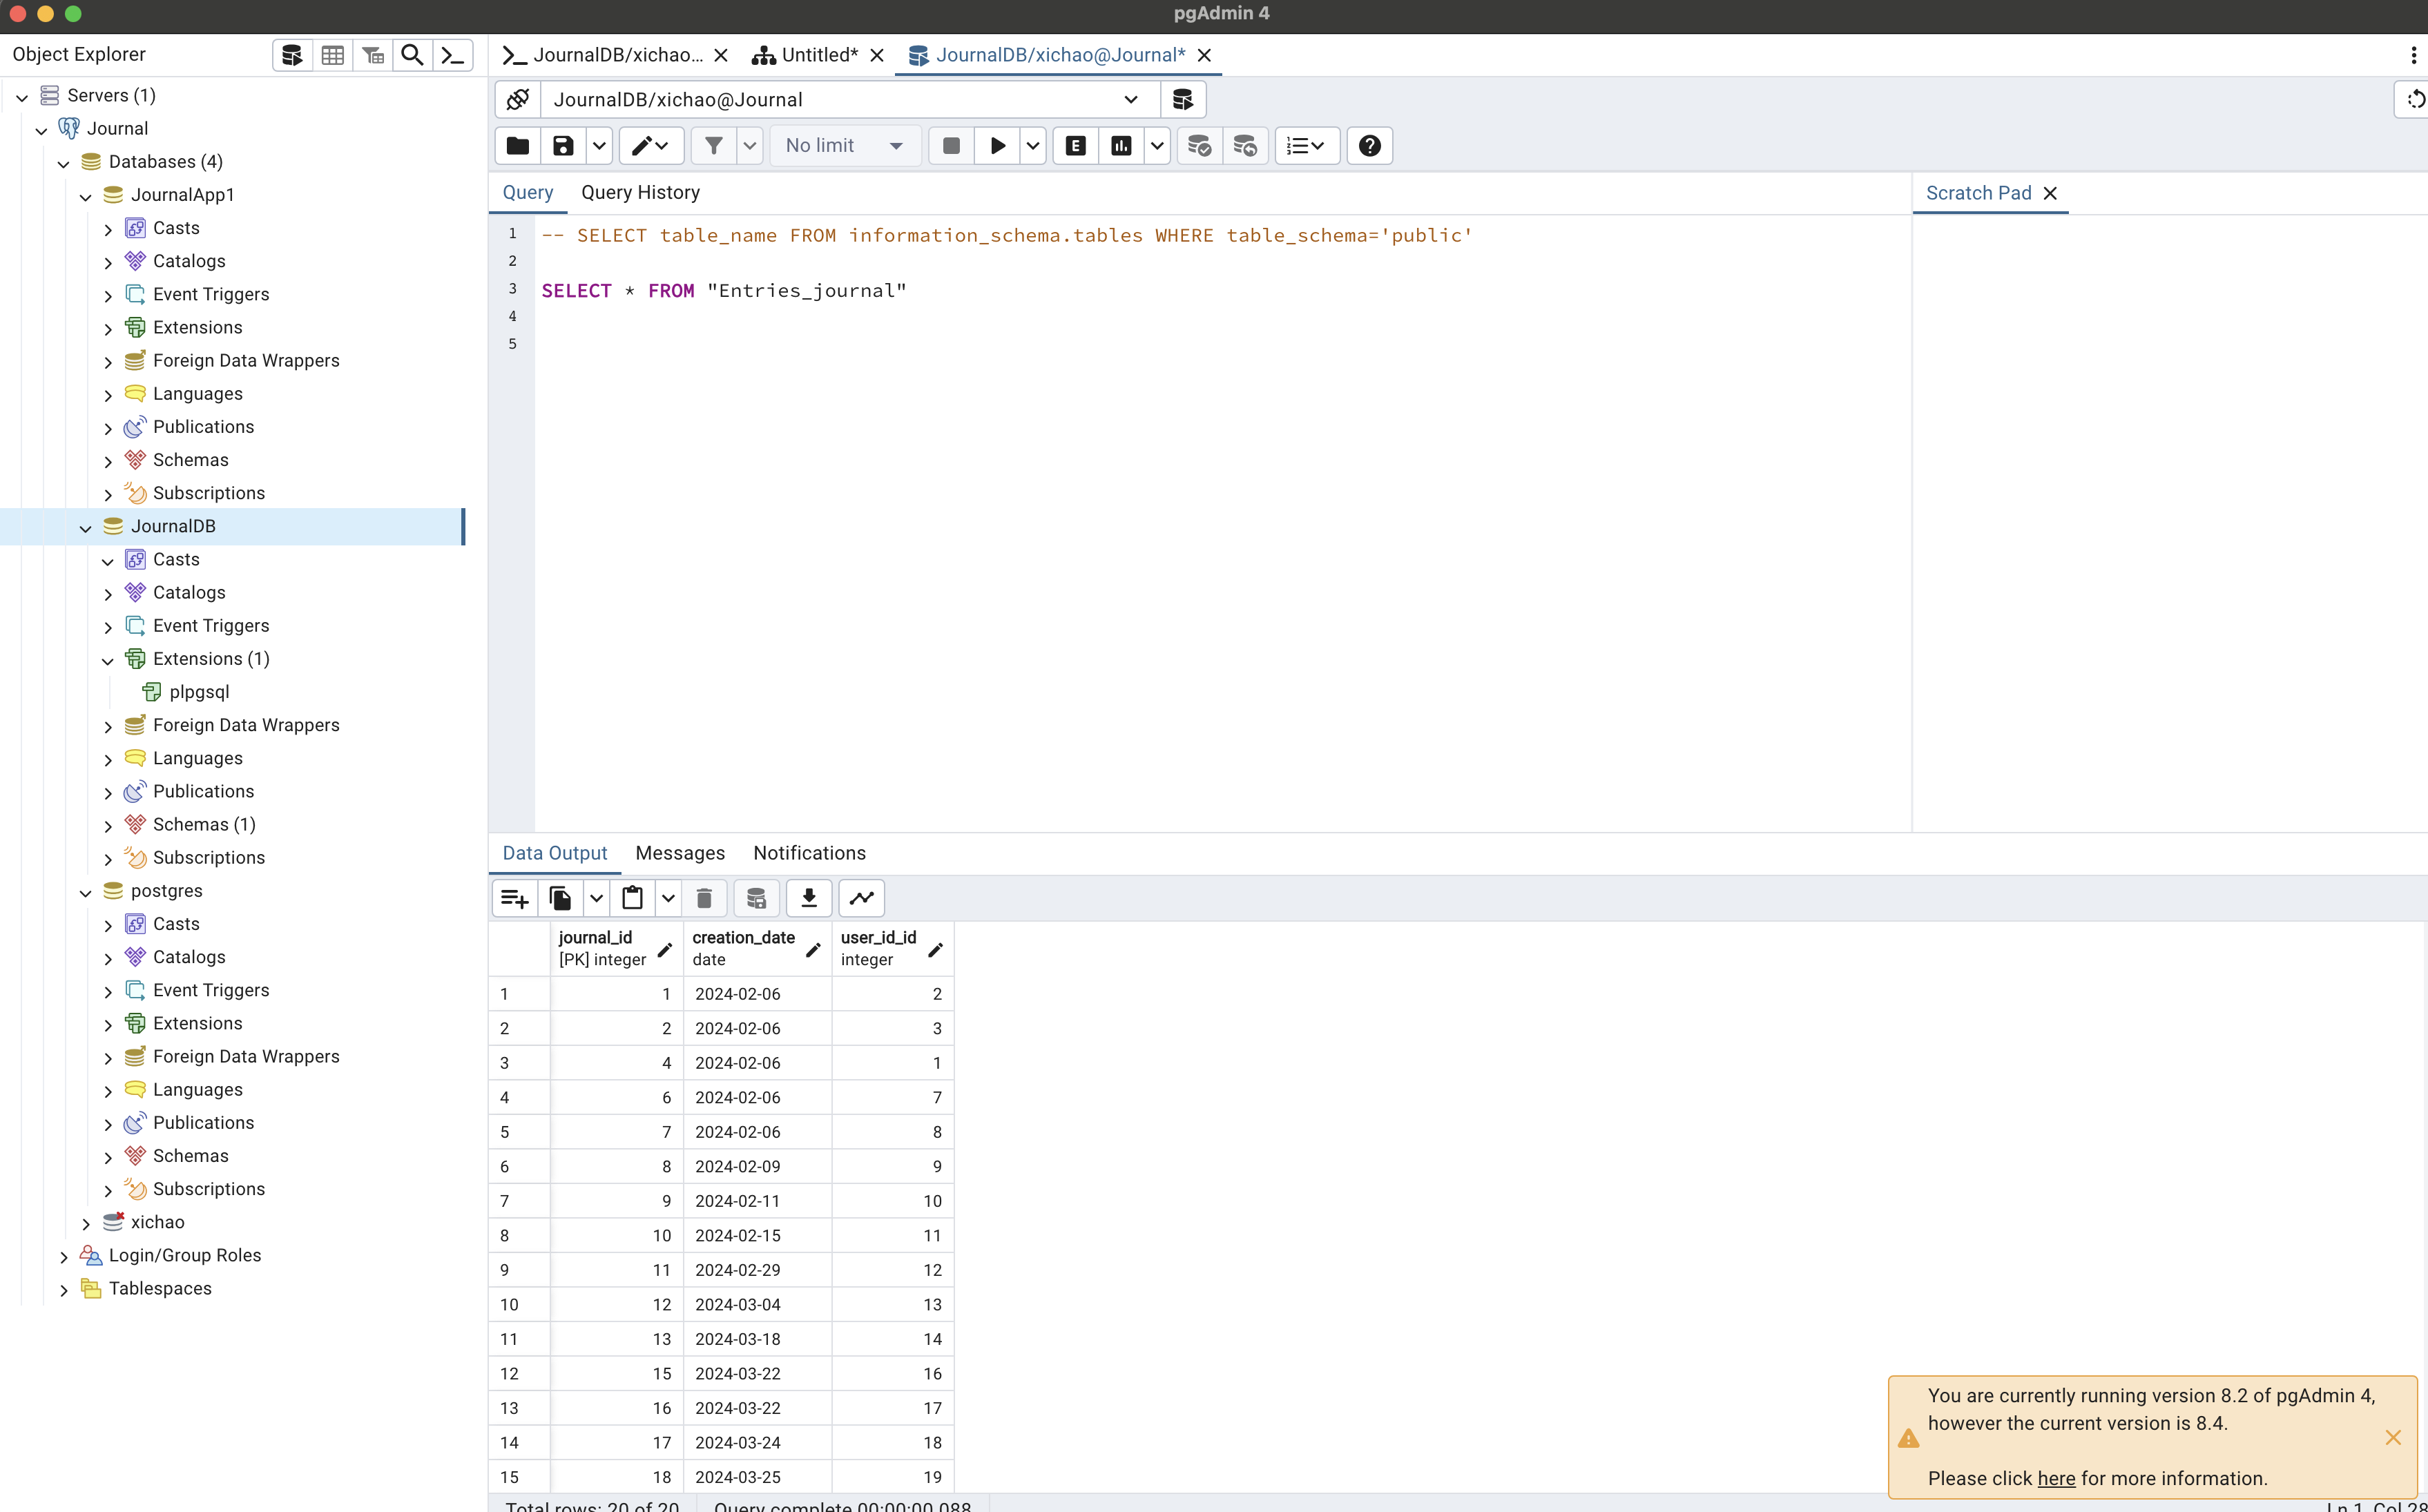
\includegraphics[width=\textwidth]{Assets/pgJournal.png}
    \caption{Journal table in the database.}
    \label{fig:pg_journal_table}
\end{figure}

\begin{figure}
    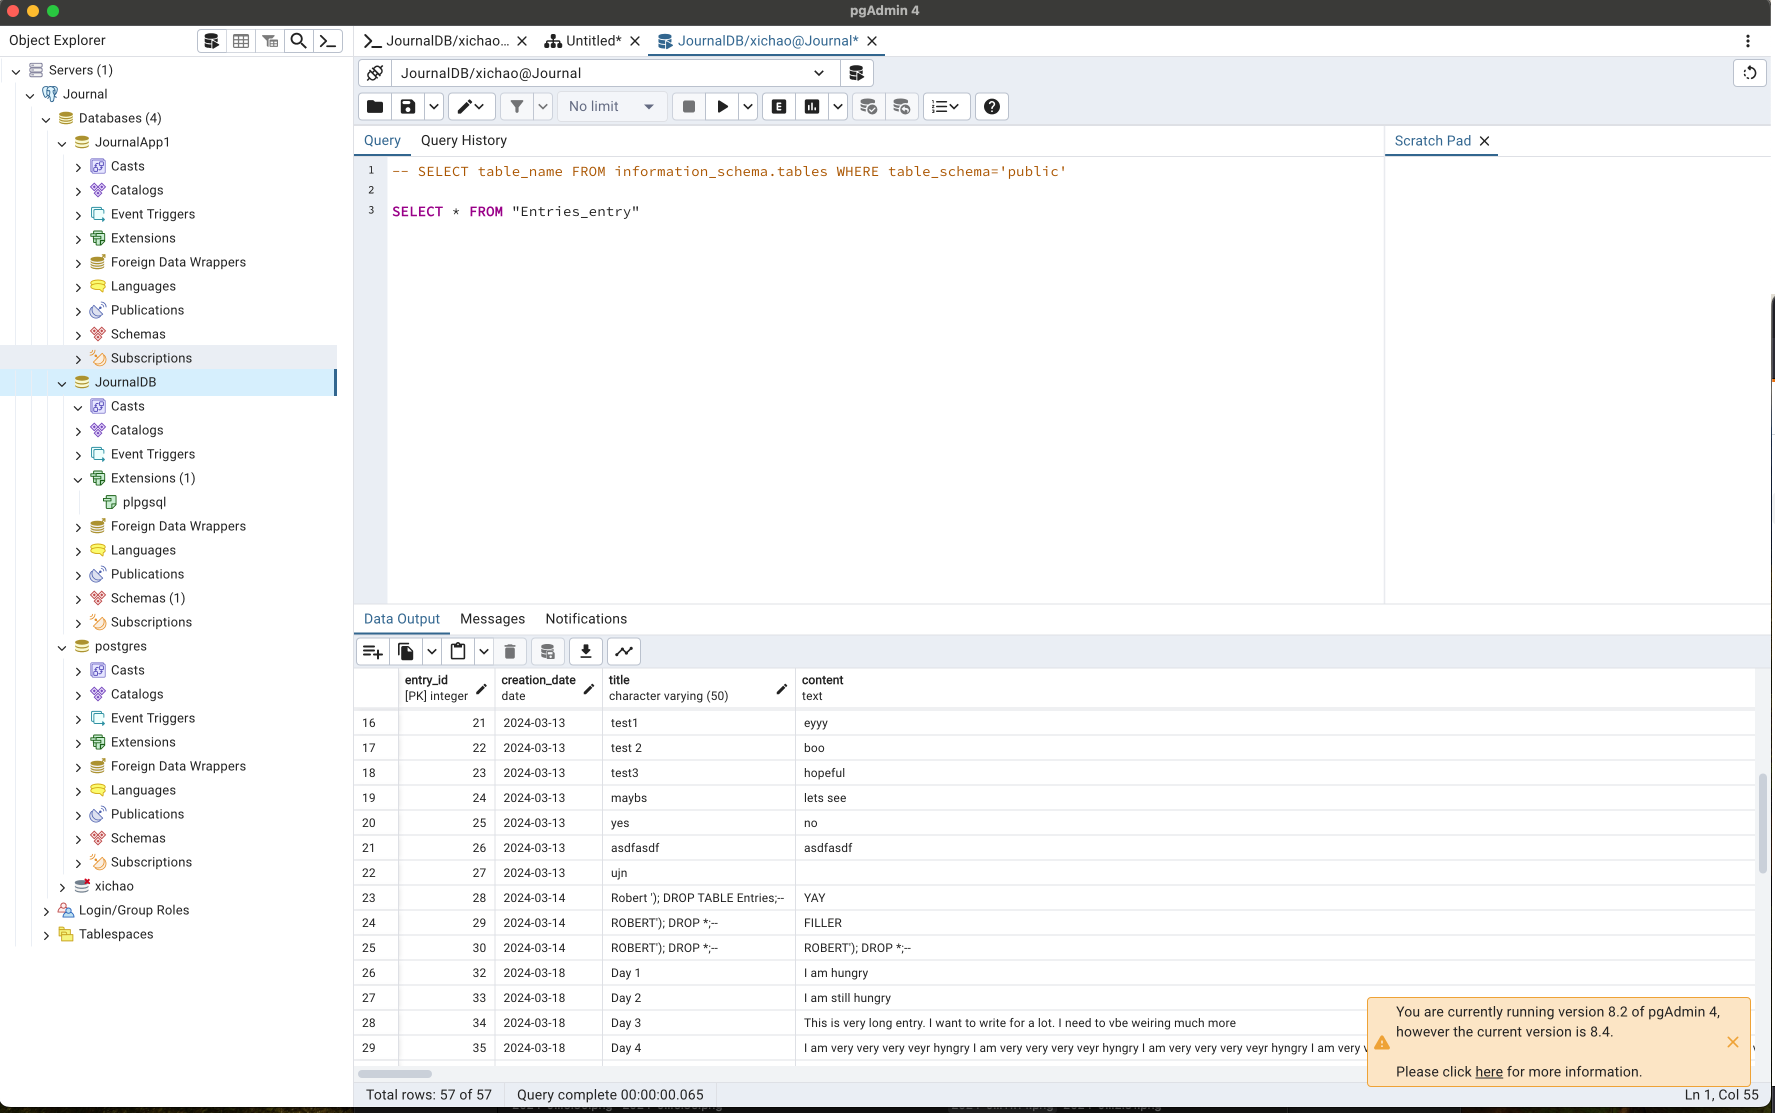
\includegraphics[width=\textwidth]{Assets/pgEntries.png}
    \caption{Entries table in the database.}
    \label{fig:pg_entry_table}
\end{figure}